\documentclass[a4paper, 10pt, colorlinks=true, linkcolor=black, urlcolor=blue, citecolor=blue, hidelinks]{article}
\usepackage{xcolor}
\definecolor{verdeBitless}{HTML}{2E8B57}
\usepackage[italian]{babel} 
\usepackage{comment}      
\setcounter{secnumdepth}{4}
\setcounter{tocdepth}{4}
\usepackage{graphicx} 
\usepackage{multirow}
\usepackage{tikz}
\usepackage{geometry}
\newcommand{\ucref}[1]{UC \ref{#1}}
\usepackage[table]{xcolor}
\usepackage{float} 
\usepackage{setspace}
\definecolor{bluBitless}{HTML}{3A75C4}
\usepackage{tabularx}
\newcolumntype{L}{>{\raggedright\arraybackslash}X}
\usepackage{fancyhdr}

\pagestyle{fancy}
\fancyhf{}
\fancyhead[L]{The Bitless}
\fancyhead[R]{Piano di Progetto}
\fancyfoot[C]{\thepage}

\usepackage{hyperref}
\hypersetup{
    colorlinks=true,
    linkcolor=black, 
    urlcolor=bluBitless,     
    citecolor=0 0 0 0,  
    filecolor=0 0 0 0,
    breaklinks=true,
    pdfpagemode=UseNone    
}

\begin{document}

\newcommand{\tipoverbale}{Piano di Progetto}
\newcommand{\dataverbale}{}
\newcommand{\dataversione}{2026-04-27}
\newcommand{\versione}{0.4.0}
\newcommand{\stato}{Stesura}
\newcommand{\destinatari}{The Bitless, prof. Tullio Vardanega, prof. Riccardo Cardin}
\def\templatedir{../../../templates}

\begin{titlepage}
\pagenumbering{gobble}
\begin{titlepage} 
      \begin{center}
            \thispagestyle{empty}
            \providecommand{\templatedir}{../../../../templates}
            
\includegraphics[width=15cm]{\templatedir/logo_gruppo.png}
            \begin{spacing}{1.2}
                \Huge{\textbf{\titolo \ \dataverbale}}
            \end{spacing}

            \vspace{2cm}


            \begin{center}
            \textbf{The Bitless} (Gruppo 18): \\
            Lorenzo Battistella (2103116), Edoardo De Piccoli (2101055), Davide Facco (2087852), \\ Anna Marini (2110986), Andrea Menegaldo (2116426), Samuele Vendramin (2111934),\\ Simone Zecchinato (2113189)
            \end{center}

            \vspace{1cm}

            \begin{center}
                \begin{tabular}{|c|c|c|c|}
                    \hline
                    \multicolumn{4}{|c|}{\textbf{Informazioni documento}} \\
                    \hline
                    \textbf{Versione} & \textbf{Data} & \textbf{Stato}  & \textbf{Destinatari} \\
                    \hline
                    \versione & \dataversione & \stato & \destinatari \\
                    \hline
                \end{tabular}
            \end{center}

            \vfill
            
            \begin{center}
                Contatti: thebitless.swe@gmail.com
            \end{center}
            
        \end{center}
    \end{titlepage}
\end{titlepage}

\pagenumbering{arabic}

\begin{center}
    \textbf{Registro delle modifiche}
\end{center}

\vspace{0.3cm}

\begin{center}
    \small
    \begin{tabularx}{\textwidth}{|c|c|L|c|c|L|}
        \hline
        \textbf{Versione} & \textbf{Data} & \textbf{Autore} & \textbf{Verificatore} & \textbf{Approvatore} & \textbf{Descrizione} \\
        \hline
        0.6.0 & 2026-05-14 & A. Marini & E. De Piccoli & - & Aaggiornamento dei contenuti dopo verifica interna \\
        \hline
        0.5.0 & 2026-05-06 & S. Vendramin & E. De Piccoli & - & Stesura Sprint \#2 e aggiornamento pianificazione attività \\
        \hline
        0.4.0 & 2026-04-27 & A. Marini & E. De Piccoli & - & Stesura Consuntivo Sprint \#1 \\
        \hline
        0.3.0 & 2026-04-21 & A. Menegaldo & E. De Piccoli & - & Stesura pianificazione Sprint \#1 \\
        \hline
        0.2.0 & 2026-04-16 & A. Marini & A. Menegaldo & - & Stesura Analisi e Gestione dei Rischi \\
        \hline
        0.1.0 & 2026-04-13 & A. Marini & A. Menegaldo & - & Struttura documento e introduzione \\
        \hline
    \end{tabularx}
\end{center}


\newpage
\pagenumbering{roman} % Numerazione romana per le pagine iniziali (opzionale)
\tableofcontents
\newpage
\newpage

\pagenumbering{arabic}


\newpage

\section{Introduzione}

\subsection{Scopo del documento}

Il Piano di Progetto rappresenta il documento di riferimento per la gestione organizzativa, temporale ed economica del progetto. 
Esso ha lo scopo di descrivere le modalità con cui il gruppo intende pianificare, coordinare e controllare le attività necessarie alla realizzazione del prodotto software.

Il documento permette di definire una visione d'insieme del lavoro da svolgere, individuando le attività principali, le risorse coinvolte, le responsabilità assegnate e le tempistiche previste. 
Inoltre, consente di monitorare l'avanzamento del progetto e di confrontare le stime iniziali con i dati effettivamente rilevati durante lo svolgimento delle attività.

Al fine di garantire un controllo efficace del progetto, il Piano di Progetto include:

\begin{itemize}
    \item l'identificazione e l'analisi dei principali rischi$_G$ di progetto; la definizione delle strategie di mitigazione dei rischi individuati;
    \item la descrizione del modello di sviluppo adottato;
    \item la pianificazione temporale delle attività;
    \item la stima dei costi e delle risorse necessarie;
    \item la definizione del preventivo e del preventivo a finire;
    \item la revisione periodica delle attività svolte e la relativa retrospettiva$_G$.
\end{itemize}

\subsection{Scopo del prodotto}

Il prodotto \textbf{Second Brain} ha lo scopo di realizzare un'applicazione web per la scrittura e la gestione di note in formato Markdown$_G$, integrando funzionalità basate su Large Language Models$_G$ per supportare l'utente nella creazione, revisione e rielaborazione dei testi.

L'applicazione si propone di offrire un editor semplice e accessibile, composto da un'area di scrittura e da una vista di anteprima renderizzata, permettendo all'utente di concentrarsi sia sulla stesura del contenuto sia sulla valutazione del risultato finale.

Attraverso l'integrazione con un LLM$_G$, il sistema deve supportare operazioni come il riassunto, la riscrittura, la traduzione, la correzione e la critica del testo secondo la metodologia dei Sei Cappelli per Pensare. Inoltre, il prodotto deve permettere la generazione automatica di un testo completo a partire da un prompt fornito dall'utente.

Lo scopo finale è verificare la potenzialità degli LLM$_G$ nell'assistere una persona nei compiti legati alla scrittura, allo sviluppo di idee e al brainstorming$_G$, realizzando uno strumento organico, semplice da utilizzare e utile anche per utenti non esperti.


\subsection{Riferimenti}

\subsubsection{Riferimenti Normativi}
\begin{itemize}
    \item \textbf{Capitolato C6 - Second Brain}: \\
    \url{https://www.math.unipd.it/~tullio/IS-1/2025/Progetto/C6.pdf} \\
    Ultimo accesso 5 aprile 2026

    \item \textbf{Regolamento del Progetto Didattico}: \\
    \url{https://www.math.unipd.it/~tullio/IS-1/2025/Dispense/PD1.pdf} \\
    Ultimo accesso 5 aprile 2026

    \item \textbf{Norme di Progetto v0.5.0}: \\
    \url{https://thebitless.github.io/RTB/doc_interna/norme-di-progetto/norme-di-progetto.pdf} \\
    Ultimo accesso 5 aprile 2026
\end{itemize}

\subsubsection{Riferimenti Informativi}
\begin{itemize}
    \item \textbf{Corso di Ingegneria del Software - I processi di ciclo di vita del software}: \\
    \url{https://www.math.unipd.it/~tullio/IS-1/2025/Dispense/T02.pdf} \\
    Ultimo accesso 5 aprile 2026

    \item \textbf{Corso di Ingegneria del Software - Modelli di sviluppo del Software}: \\
    \url{https://www.math.unipd.it/~tullio/IS-1/2025/Dispense/T03.pdf} \\
    Ultimo accesso 5 aprile 2026

    \item \textbf{Corso di Ingegneria del Software - Gestione di Progetto}: \\
    \url{https://www.math.unipd.it/~tullio/IS-1/2025/Dispense/T04.pdf} \\
    Ultimo accesso 5 aprile 2026

    \item \textbf{Glossario v0.5.0}: \\
    \url{https://thebitless.github.io/RTB/doc_interna/glossario/glossario.pdf} \\
    Ultimo accesso 5 aprile 2026
\end{itemize}

\subsection{Glossario}

Per garantire una comprensione uniforme dei termini utilizzati nella documentazione, il gruppo mette a disposizione un \textbf{Glossario}. Questo documento raccoglie le definizioni dei termini tecnici, degli acronimi e delle espressioni che potrebbero risultare ambigue o assumere un significato specifico nel contesto del progetto.

All'interno dei documenti, i termini presenti nel Glossario vengono indicati mediante una formattazione dedicata, ovvero con la lettera \textit{G} posta in pedice. Tale convenzione permette al lettore di riconoscere facilmente i concetti definiti formalmente e favorisce l'uso coerente del linguaggio in tutta la documentazione prodotta.

\subsection{Note organizzative}

Il presente documento è soggetto ad aggiornamenti periodici, in modo da rispecchiare l'evoluzione del progetto e le decisioni assunte dal gruppo nel corso delle diverse attività. La sua revisione continua consente di mantenere allineata la pianificazione con lo stato effettivo dei lavori e di controllare con maggiore precisione l'avanzamento complessivo.

Ogni modifica rilevante viene riportata nel Registro delle modifiche, così da conservare una traccia chiara delle revisioni effettuate, dei responsabili coinvolti e dello stato di maturazione del documento.

\newpage

\section{Analisi e Gestione dei Rischi}

\subsection{Introduzione}

L'attività di analisi dei rischi\textsubscript{G} ha l'obiettivo di identificare, valutare e gestire preventivamente quegli eventi che potrebbero compromettere il corretto svolgimento dei task\textsubscript{G} e il raggiungimento degli obiettivi prestabiliti. 
Per ogni rischio individuato, il gruppo ne valuta la \textbf{probabilità} di occorrenza e la \textbf{gravità} dell'impatto, definendo specifiche contromisure per mitigarli.

I rischi sono identificati tramite una sigla univoca così composta: \\
\centerline{\textbf{R[Tipo]-[Numero]}}
\begin{itemize}
    \item \textbf{R}: indica che si tratta di un Rischio\textsubscript{G};
    \item \textbf{Tipo}: rappresenta la categoria del rischio:
    \begin{itemize}
        \item \textbf{T}: Tecnologico;
        \item \textbf{O}: Organizzativo;
        \item \textbf{P}: Relativo al Prodotto.
    \end{itemize}
    \item \textbf{Numero}: identificativo numerico progressivo all'interno della categoria.
\end{itemize}


\subsection{Rischi tecnologici}

\subsubsection{RT-1: Scarsa esperienza con le tecnologie utilizzate}

\begin{itemize}
    \item \textbf{Codice:} RT-1

    \item \textbf{Nome:} Scarsa esperienza con le tecnologie utilizzate

    \item \textbf{Descrizione:} Il gruppo potrebbe incontrare difficoltà nell'utilizzo di alcune tecnologie fondamentali per lo sviluppo del prodotto \textit{Second Brain}. In particolare, il rischio riguarda Python\textsubscript{G} per la componente back-end, React\textsubscript{G} per la realizzazione dell'interfaccia utente, le API\textsubscript{G} per l'interazione con gli LLM\textsubscript{G} e la gestione del rendering Markdown\textsubscript{G}. La limitata familiarità iniziale con tali tecnologie potrebbe causare rallentamenti nelle attività di progettazione, sviluppo e integrazione, soprattutto nelle prime fasi del progetto.

    \item \textbf{Strategie di rilevamento:} Il Responsabile monitora periodicamente l'avanzamento dei task\textsubscript{G} assegnati, verificando eventuali ritardi riconducibili a difficoltà tecniche. Durante gli sprint\textsubscript{G}, il gruppo raccoglie feedback dai singoli membri per individuare tempestivamente eventuali lacune. L'utilizzo di GitHub\textsubscript{G} e dell'integrazione continua permette inoltre di rilevare errori ricorrenti nell'uso delle tecnologie adottate, specialmente durante le fasi di integrazione tra front-end, back-end e servizi LLM\textsubscript{G}.

    \item \textbf{Contromisure:} Il gruppo prevede attività di studio e momenti di condivisione interna sulle tecnologie meno note. I membri con maggiore esperienza supportano chi incontra difficoltà, in particolare nelle attività più delicate, come la configurazione dell'ambiente di sviluppo, l'integrazione con le API\textsubscript{G} degli LLM\textsubscript{G} e la gestione del rendering Markdown\textsubscript{G}. In caso di dubbi sulle tecnologie proposte o sulle modalità di integrazione, il team potrà richiedere chiarimenti alla Proponente\textsubscript{G}. Qualora una tecnologia risultasse poco adatta o troppo onerosa, potranno essere valutate soluzioni alternative compatibili con il capitolato C6.

    \item \textbf{Probabilità:} Alta

    \item \textbf{Pericolosità:} Alta
\end{itemize}


\subsubsection{RT-2: Scarsa esperienza nell'utilizzo degli strumenti di sviluppo}

\begin{itemize}
    \item \textbf{Codice:} RT-2

    \item \textbf{Nome:} Scarsa esperienza nell'utilizzo degli strumenti di sviluppo

    \item \textbf{Descrizione:} Il gruppo potrebbe incontrare difficoltà nell'utilizzo corretto degli strumenti a supporto dello sviluppo, della documentazione e della gestione del progetto. In particolare, il rischio riguarda l'uso di GitHub\textsubscript{G} per il versionamento del codice e della documentazione, la gestione di branch\textsubscript{G}, pull request\textsubscript{G}, issue\textsubscript{G} e milestone\textsubscript{G}, oltre alla produzione della documentazione in LaTeX\textsubscript{G}. Una gestione non uniforme di tali strumenti potrebbe causare conflitti tra versioni, errori di integrazione, rallentamenti nella revisione del lavoro e difficoltà nel mantenere allineati prodotto software e documentazione.

    \item \textbf{Strategie di rilevamento:} Il Responsabile controlla periodicamente l'utilizzo degli strumenti condivisi, verificando la corretta apertura e chiusura delle issue\textsubscript{G}, l'aggiornamento delle attività assegnate e la coerenza tra branch\textsubscript{G}, pull request\textsubscript{G} e versioni dei documenti. Durante gli sprint\textsubscript{G}, il gruppo monitora eventuali errori ricorrenti nei commit\textsubscript{G}, nei merge\textsubscript{G} e nella compilazione della documentazione. Le difficoltà vengono inoltre rilevate attraverso il confronto interno durante le riunioni di coordinamento.

    \item \textbf{Contromisure:} Il gruppo definisce procedure operative comuni all'interno delle Norme di Progetto\textsubscript{G}, così da uniformare l'uso degli strumenti e ridurre ambiguità nel modo di lavorare. Vengono predisposti template\textsubscript{G} per documenti, issue\textsubscript{G}, pull request\textsubscript{G} e verbali, in modo da rendere più semplice e controllabile il lavoro dei singoli membri. I membri con maggiore esperienza affiancano chi incontra difficoltà, specialmente nelle attività più delicate come merge\textsubscript{G}, rilascio delle versioni e aggiornamento del sito pubblico.

    \item \textbf{Probabilità:} Media

    \item \textbf{Pericolosità:} Media
\end{itemize}


\subsubsection{RT-3: Presenza di errori nel codice}

\begin{itemize}
    \item \textbf{Codice:} RT-3

    \item \textbf{Nome:} Presenza di errori nel codice

    \item \textbf{Descrizione:} Durante lo sviluppo del prodotto \textit{Second Brain} potrebbero essere introdotti errori nel codice, dovuti alla complessità dell'integrazione tra le diverse componenti del sistema. Il rischio riguarda in particolare la comunicazione tra front-end React\textsubscript{G} e back-end Python\textsubscript{G}, l'interazione con le API\textsubscript{G} degli LLM\textsubscript{G}, la gestione del testo Markdown\textsubscript{G}, il salvataggio delle note e l'eventuale persistenza server-side. Alcuni difetti potrebbero non emergere immediatamente durante la scrittura del codice, ma solo in fase di test\textsubscript{G}, integrazione o utilizzo del prodotto, causando ritardi nelle attività pianificate.

    \item \textbf{Strategie di rilevamento:} Il gruppo rileva questo rischio attraverso l'esecuzione periodica di test\textsubscript{G}, la revisione del codice e il controllo delle funzionalità implementate rispetto ai casi d'uso\textsubscript{G} e ai requisiti individuati. Le pull request\textsubscript{G} vengono verificate prima dell'integrazione nel branch\textsubscript{G} principale, così da individuare errori logici, problemi di compatibilità o regressioni. Particolare attenzione viene posta alle funzionalità più critiche, come l'invio di richieste agli LLM\textsubscript{G}, la gestione degli errori di risposta, il salvataggio dei dati e il corretto aggiornamento dell'interfaccia utente.

    \item \textbf{Contromisure:} Per ridurre l'impatto del rischio, il gruppo adotta una strategia di sviluppo incrementale, evitando di integrare grandi quantità di codice non verificato. Ogni funzionalità viene testata prima dell'integrazione definitiva e, in caso di errore, il componente responsabile procede inizialmente con l'analisi e la correzione del problema. Se l'anomalia risulta complessa, viene richiesto il supporto dei membri più esperti del team. In presenza di errori critici, il gruppo dà priorità al debugging\textsubscript{G} e può riorganizzare la pianificazione, posticipando attività secondarie per preservare la stabilità del prodotto.

    \item \textbf{Probabilità:} Alta

    \item \textbf{Pericolosità:} Media
\end{itemize}

\subsection{Rischi organizzativi}

\subsubsection{RO-1: Periodi di rallentamento}

\begin{itemize}
    \item \textbf{Codice:} RO-1

    \item \textbf{Nome:} Periodi di rallentamento

    \item \textbf{Descrizione:} Il gruppo potrebbe subire rallentamenti nello svolgimento delle attività a causa di periodi dell'anno caratterizzati da minore disponibilità dei membri, come festività, sessioni d'esame e vacanze estive. Tale rischio può incidere sull'avanzamento del progetto \textit{Second Brain}, soprattutto nelle fasi in cui sono richieste attività coordinate tra più componenti del team. Se non gestito correttamente, il rallentamento potrebbe compromettere il rispetto delle scadenze pianificate e ridurre il margine disponibile per correzioni o attività di verifica.

    \item \textbf{Strategie di rilevamento:} Il Responsabile monitora periodicamente le ore rendicontate dai membri del gruppo e confronta l'avanzamento effettivo dei task\textsubscript{G} con quanto previsto dalla pianificazione dello sprint\textsubscript{G}. Particolare attenzione viene posta ai periodi in cui è prevedibile una minore disponibilità, come festività, sessioni d'esame e vacanze. Durante le riunioni interne, il team verifica eventuali ritardi, attività bloccate o carichi di lavoro non sostenibili, così da individuare tempestivamente situazioni che potrebbero influire sulla consegna degli incrementi previsti.

    \item \textbf{Contromisure:} La pianificazione del progetto tiene conto dei periodi di minore disponibilità, distribuendo le attività più critiche nei momenti in cui il gruppo può garantire maggiore continuità di lavoro. In caso di rallentamenti, il Responsabile può riassegnare i task\textsubscript{G}, anticipare attività meno dipendenti da altri membri oppure posticipare attività secondarie, dando priorità agli elementi necessari per rispettare gli obiettivi del capitolato C6 e mantenere stabile l'avanzamento del prodotto.
    \item \textbf{Periodi critici previsti:}
    \begin{center}
        \renewcommand{\arraystretch}{1.3}
        \begin{tabularx}{0.9\textwidth}{|l|X|}
            \hline
            \textbf{Periodo} & \textbf{Motivazione} \\
            \hline
            Periodo pasquale & Possibile riduzione della disponibilità dovuta a festività e spostamenti personali. \\
            \hline
            Sessione estiva & Possibile sovrapposizione tra attività di progetto, studio individuale ed esami universitari. \\
            \hline
            Agosto & Possibile rallentamento generale dovuto a vacanze e minore reperibilità dei membri del gruppo. \\
            \hline
        \end{tabularx}
    \end{center}

    \item \textbf{Probabilità:} Media

    \item \textbf{Pericolosità:} Alta
\end{itemize}

\subsubsection{RO-2: Incomprensioni comunicative}

\begin{itemize}
    \item \textbf{Codice:} RO-2

    \item \textbf{Nome:} Incomprensioni comunicative

    \item \textbf{Descrizione:} Il gruppo potrebbe incontrare difficoltà nella comunicazione interna, con il rischio che alcune informazioni vengano trasmesse in modo incompleto, poco chiaro o non uniforme tra i membri del team. Questo potrebbe portare a interpretazioni diverse degli obiettivi del progetto, dei requisiti del capitolato C6 o delle attività assegnate durante gli sprint\textsubscript{G}. 

    \item \textbf{Strategie di rilevamento:} Tutti i componenti del gruppo sono tenuti a collaborare attivamente nel rilevare eventuali dubbi, ambiguità o disallineamenti informativi. Durante gli incontri interni, ciascun membro può segnalare difficoltà nella comprensione dei task\textsubscript{G}, delle decisioni prese o delle responsabilità assegnate. Il gruppo monitora inoltre lo stato delle issue\textsubscript{G}, dei verbali, delle attività pianificate e dell'avanzamento dei lavori, così da individuare tempestivamente eventuali incoerenze tra quanto deciso e quanto effettivamente svolto. Il Responsabile mantiene una funzione di coordinamento, ma il controllo della chiarezza comunicativa è condiviso da tutto il team.

    \item \textbf{Contromisure:} Il gruppo utilizza canali di comunicazione ufficiali e condivisi, evitando che decisioni importanti rimangano disperse in conversazioni informali o private. Ogni riunione viene accompagnata da un verbale in cui vengono riportate decisioni, responsabilità assegnate, scadenze e problemi emersi. I membri del team sono invitati a chiedere chiarimenti appena rilevano dubbi, senza attendere fasi successive dello sprint\textsubscript{G}. Le decisioni tecniche e organizzative rilevanti vengono documentate nelle Norme di Progetto\textsubscript{G} o nei documenti opportuni, così da mantenere una fonte comune e consultabile.

    \item \textbf{Probabilità:} Media

    \item \textbf{Pericolosità:} Media
\end{itemize}

\subsubsection{RO-5: Scarsa esperienza nel lavoro di gruppo}

\begin{itemize}
    \item \textbf{Codice:} RO-5

    \item \textbf{Nome:} Scarsa esperienza nel lavoro di gruppo

    \item \textbf{Descrizione:} Il gruppo potrebbe incontrare difficoltà nella gestione collaborativa di un progetto software complesso come \textit{Second Brain}, che richiede coordinamento tra attività di analisi, progettazione, sviluppo, verifica e documentazione. La presenza di componenti diverse, come interfaccia React\textsubscript{G}, back-end Python\textsubscript{G}, integrazione con API\textsubscript{G} di LLM\textsubscript{G}, gestione delle note e produzione della documentazione, rende necessario un lavoro organizzato e coerente tra tutti i membri. Una scarsa esperienza nel lavoro di gruppo potrebbe causare sovrapposizioni nei task\textsubscript{G}, distribuzione non equilibrata delle attività, difficoltà nell'integrazione del codice o ritardi nella consegna degli incrementi previsti.

    \item \textbf{Strategie di rilevamento:} Il gruppo monitora periodicamente l'avanzamento delle attività assegnate, verificando che ogni membro abbia compreso il proprio compito e che non vi siano sovrapposizioni o attività lasciate scoperte. Durante le riunioni interne vengono discussi lo stato dei task\textsubscript{G}, eventuali blocchi, problemi di coordinamento e difficoltà nell'integrazione del lavoro svolto. L'utilizzo di issue\textsubscript{G}, milestone\textsubscript{G}, branch\textsubscript{G} e pull request\textsubscript{G} consente inoltre di individuare tempestivamente disallineamenti tra le attività pianificate e quelle realmente completate.

    \item \textbf{Contromisure:} Il gruppo definisce nelle Norme di Progetto\textsubscript{G} un workflow\textsubscript{G} condiviso, così da stabilire regole comuni per assegnazione dei task\textsubscript{G}, gestione dei branch\textsubscript{G}, apertura delle pull request\textsubscript{G}, revisione del lavoro e integrazione degli incrementi. Le attività vengono suddivise in modo chiaro e tracciabile, evitando che più persone lavorino inconsapevolmente sulla stessa parte o che alcune sezioni del progetto rimangano prive di responsabili operativi. Tutti i membri sono tenuti a comunicare difficoltà, ritardi o dubbi appena emergono, collaborando attivamente alla risoluzione dei problemi. In caso di attività particolarmente critiche, il gruppo può prevedere lavoro a coppie, revisioni incrociate o supporto da parte dei componenti con maggiore familiarità rispetto all'area interessata.

    \item \textbf{Probabilità:} Media

    \item \textbf{Pericolosità:} Media
\end{itemize}

\subsubsection{RO-6: Errori di pianificazione}

\begin{itemize}
    \item \textbf{Codice:} RO-6

    \item \textbf{Nome:} Errori di pianificazione

    \item \textbf{Descrizione:} Il gruppo potrebbe pianificare in modo non adeguato le attività necessarie allo sviluppo di \textit{Second Brain}, sottostimando la complessità di alcuni task\textsubscript{G} o non considerando correttamente le dipendenze tra le diverse parti del progetto. Questo rischio può riguardare, ad esempio, l'integrazione tra front-end React\textsubscript{G}, back-end Python\textsubscript{G}, API\textsubscript{G} degli LLM\textsubscript{G}, gestione della persistenza, rendering Markdown\textsubscript{G}, test e documentazione. Una pianificazione poco precisa potrebbe causare ritardi, sovraccarico di alcuni membri, attività svolte in ordine non ottimale o difficoltà nel rispettare le scadenze previste.

    \item \textbf{Strategie di rilevamento:} Il gruppo controlla periodicamente l'avanzamento delle attività confrontando quanto pianificato con quanto effettivamente completato. Durante le riunioni interne vengono analizzati eventuali scostamenti rispetto alle stime iniziali, task\textsubscript{G} bloccati, dipendenze non considerate o attività che richiedono più tempo del previsto. L'utilizzo di issue\textsubscript{G}, milestone\textsubscript{G} e strumenti di tracciamento permette di individuare tempestivamente ritardi o squilibri nella distribuzione del lavoro.

    \item \textbf{Contromisure:} La pianificazione viene riesaminata a ogni sprint\textsubscript{G}, così da correggere eventuali stime troppo ottimistiche e adattare il piano allo stato reale del progetto. Il gruppo mantiene margini di flessibilità nella suddivisione delle attività, dando priorità ai requisiti obbligatori e alle componenti più critiche del capitolato C6. Tutti i membri collaborano alla revisione delle stime, segnalando tempestivamente difficoltà, dipendenze non previste o carichi di lavoro eccessivi. In caso di ritardi, il gruppo può riassegnare alcune attività, ridurre temporaneamente il lavoro su funzionalità opzionali o riorganizzare le priorità per garantire il completamento degli obiettivi principali.

    \item \textbf{Probabilità:} Bassa

    \item \textbf{Pericolosità:} Alta
\end{itemize}

\subsubsection{RO-7: Rotazione dei ruoli}

\begin{itemize}
    \item \textbf{Codice:} RO-7

    \item \textbf{Nome:} Rotazione dei ruoli

    \item \textbf{Descrizione:} Ogni componente del gruppo deve ricoprire, a rotazione, i diversi ruoli previsti dal regolamento del progetto. Questa modalità di lavoro può generare difficoltà organizzative, soprattutto all'inizio di ogni sprint\textsubscript{G}, quando un membro assume un ruolo con cui ha poca esperienza o deve proseguire attività precedentemente gestite da altri. Nel caso del progetto \textit{Second Brain}, questo rischio può incidere sia sulle attività tecniche, come sviluppo front-end React\textsubscript{G}, back-end Python\textsubscript{G} e integrazione con API\textsubscript{G} LLM\textsubscript{G}, sia sulle attività documentali e di verifica. L'impatto può aumentare nel tempo, poiché il materiale prodotto diventa progressivamente più ampio e complesso da comprendere, controllare e aggiornare.

    \item \textbf{Strategie di rilevamento:} Il gruppo verifica periodicamente se il cambio di ruolo sta causando rallentamenti, dubbi operativi o difficoltà nella presa in carico delle attività. Durante le riunioni di pianificazione e retrospettiva vengono raccolti feedback dai membri che hanno cambiato ruolo, così da individuare eventuali problemi ricorrenti. La rendicontazione delle ore, l'avanzamento dei task\textsubscript{G} e lo stato delle issue\textsubscript{G} permettono inoltre di riconoscere tempestivamente eventuali squilibri o ritardi legati alla rotazione.

    \item \textbf{Contromisure:} Le Norme di Progetto\textsubscript{G} definiscono in modo chiaro le responsabilità associate a ciascun ruolo, così da ridurre ambiguità durante il passaggio da uno sprint\textsubscript{G} al successivo. Prima di ogni rotazione, il membro uscente deve lasciare indicazioni comprensibili sul lavoro svolto, sui problemi aperti e sulle attività ancora da completare. Durante le riunioni interne, il gruppo dedica tempo al passaggio di consegne e alla chiarificazione dei compiti assegnati. In caso di difficoltà, i membri con maggiore familiarità con un ruolo o con una specifica attività supportano chi subentra, evitando che la rotazione comprometta la continuità del lavoro.

    \item \textbf{Probabilità:} Alta

    \item \textbf{Pericolosità:} Alta
\end{itemize}

\subsubsection{RO-8: Errata stima delle attività}

\begin{itemize}
    \item \textbf{Codice:} RO-8

    \item \textbf{Nome:} Errata stima delle attività

    \item \textbf{Descrizione:} Il gruppo potrebbe sottostimare o sovrastimare il tempo, le risorse o la complessità necessari per completare alcune attività del progetto. Nel caso del prodotto \textit{Second Brain}, questo rischio può riguardare sia attività di sviluppo, come l'integrazione con gli LLM\textsubscript{G}, la gestione del rendering Markdown\textsubscript{G} o la persistenza delle note, sia attività documentali e di verifica. Una sottostima può causare ritardi e sovraccarico di lavoro, mentre una sovrastima può portare a una pianificazione poco efficiente delle risorse disponibili.

    \item \textbf{Strategie di rilevamento:} Il gruppo confronta periodicamente le ore preventivate con quelle effettivamente impiegate per ciascun task\textsubscript{G}. Durante le riunioni di avanzamento e retrospettiva vengono analizzati eventuali scostamenti significativi rispetto alla pianificazione iniziale, così da individuare attività più complesse o più semplici del previsto.

    \item \textbf{Contromisure:} Il gruppo aggiorna la pianificazione in modo incrementale, correggendo le stime sulla base dei dati raccolti durante gli sprint\textsubscript{G}. Le attività più incerte vengono suddivise in task\textsubscript{G} più piccoli e controllabili. In caso di sottostima, il gruppo può ridefinire le priorità, riallocare le risorse o posticipare attività meno urgenti. In caso di sovrastima, il tempo disponibile può essere destinato al miglioramento della qualità, alla verifica o alla documentazione.

    \item \textbf{Probabilità:} Media

    \item \textbf{Pericolosità:} Alta
\end{itemize}

\subsection{Rischi relativi al prodotto}

\subsubsection{RP-1: Errata comprensione del capitolato}

\begin{itemize}
    \item \textbf{Codice:} RP-1

    \item \textbf{Nome:} Errata comprensione del capitolato

    \item \textbf{Descrizione:} Il gruppo potrebbe interpretare in modo non corretto alcuni requisiti\textsubscript{G} presenti nel capitolato\textsubscript{G} C6 - \textit{Second Brain}, oppure non individuare correttamente alcune funzionalità richieste dalla Proponente\textsubscript{G}. Questo rischio potrebbe portare alla realizzazione di un prodotto non pienamente conforme alle aspettative, soprattutto per quanto riguarda l'integrazione con gli LLM\textsubscript{G}, il supporto a Markdown\textsubscript{G}, la gestione delle note e le funzionalità opzionali come persistenza server-side, collegamento tra note e RAG\textsubscript{G}.

    \item \textbf{Strategie di rilevamento:} Il gruppo verifica periodicamente la coerenza tra requisiti\textsubscript{G}, casi d'uso\textsubscript{G} e contenuto del capitolato\textsubscript{G}. Durante le riunioni interne vengono discussi eventuali punti ambigui e confrontate le interpretazioni dei membri del team. Inoltre, il documento di Analisi dei Requisiti viene aggiornato in modo incrementale per correggere eventuali imprecisioni emerse durante l'avanzamento del progetto.

    \item \textbf{Contromisure:} In presenza di dubbi o ambiguità, il gruppo si impegna a contattare la Proponente\textsubscript{G} per ottenere chiarimenti ufficiali. Viene inoltre mantenuta una tracciabilità esplicita tra requisiti\textsubscript{G}, fonti e casi d'uso\textsubscript{G}, così da ridurre il rischio di introdurre funzionalità non richieste o di trascurare elementi obbligatori. Le dispense del corso e il regolamento del progetto vengono utilizzati come supporto metodologico per svolgere correttamente l'analisi.

    \item \textbf{Probabilità:} Bassa

    \item \textbf{Pericolosità:} Media
\end{itemize}



\subsection{Tabella riassuntiva dei rischi}
Nella seguente tabella vengono riepilogati tutti i rischi individuati, indicando per ciascuno il codice, il nome, la probabilità di occorrenza e la pericolosità.

\begin{table}[H]
    \centering
    \renewcommand{\arraystretch}{1.5}
    \begin{tabularx}{\textwidth}{|c|L|c|c|}
        \hline
        \rowcolor{bluBitless!8}
        \textbf{Codice} & \textbf{Nome del Rischio} & \textbf{Probabilità} & \textbf{Pericolosità} \\
        \hline
        \textbf{RT-1} & Rischio legato all'utilizzo delle tecnologie & Media & Alta \\
        \hline
        \textbf{RT-2} & Rischio legato all'utilizzo degli strumenti di sviluppo & Bassa & Media \\
        \hline
        \textbf{RT-3} & Rischio legato agli errori nel codice & Alta & Media \\
        \hline
        \textbf{RO-1} & Rischio legato agli impegni accademici & Media & Media \\
        \hline
        \textbf{RO-2} & Rischio legato alle contingenze personali & Bassa & Media \\
        \hline
        \textbf{RO-3} & Rischio legato alle incomprensioni comunicative & Bassa & Media \\
        \hline
        \textbf{RO-4} & Rischio legato ai contrasti interni & Bassa & Bassa \\
        \hline
        \textbf{RO-5} & Rischio legato alla scarsa esperienza nel lavoro di gruppo & Media & Media \\
        \hline
        \textbf{RO-6} & Rischio legato agli errori di pianificazione & Bassa & Alta \\
        \hline
        \textbf{RP-1} & Rischio legato alla malcomprensione del capitolato & Bassa & Alta \\
        \hline
        \textbf{RP-2} & Rischio legato alla sottostima o sovrastima delle attività & Media & Media \\
        \hline
        \textbf{RP-3} & Rischio legato alla mancanza di supporto esecutivo & Bassa & Media \\
        \hline
    \end{tabularx}
    \caption{Tabella riassuntiva dei rischi individuati}
\end{table}

\section{Modello di sviluppo}

Per lo sviluppo del prodotto \textit{Second Brain}, il gruppo ha scelto di adottare un modello di sviluppo di tipo Agile\textsubscript{G}. Tale scelta è motivata dalla necessità di mantenere un'elevata flessibilità durante l'intero ciclo di vita del progetto, permettendo al team di adattarsi progressivamente a nuove esigenze, chiarimenti della Proponente\textsubscript{G} e possibili modifiche nella comprensione del capitolato\textsubscript{G}.

Il gruppo ha deciso di organizzare il lavoro in sprint\textsubscript{G}, ovvero periodi di durata prestabilita, generalmente pari a due settimane. Ogni sprint\textsubscript{G} prevede la selezione di un insieme di attività da completare, in modo da produrre un incremento verificabile del prodotto o della documentazione.

Nello specifico, il gruppo si ispira ad alcuni eventi del framework Scrum\textsubscript{G}, adattandoli al contesto del progetto didattico:

\begin{itemize}
    \item \textbf{Sprint Planning:} all'inizio di ogni sprint\textsubscript{G}, il gruppo analizza le attività presenti nel backlog\textsubscript{G} e seleziona quelle da svolgere durante l'iterazione. I task\textsubscript{G} vengono assegnati ai membri del team tenendo conto delle priorità, delle dipendenze tra attività e della disponibilità oraria di ciascun componente;

    \item \textbf{Sprint Review:} al termine dello sprint\textsubscript{G}, il gruppo valuta il lavoro completato e verifica se gli obiettivi stabiliti siano stati raggiunti. In questa fase vengono discussi gli incrementi prodotti, eventuali difficoltà incontrate e possibili dubbi da sottoporre alla Proponente\textsubscript{G};

    \item \textbf{Sprint Retrospective:} dopo la revisione dello sprint\textsubscript{G}, il gruppo analizza l'andamento dell'iterazione dal punto di vista organizzativo. Vengono individuati gli aspetti positivi, le criticità emerse e le azioni correttive da applicare negli sprint\textsubscript{G} successivi.
\end{itemize}

A ogni nuova iterazione viene inoltre pianificata la rotazione dei ruoli prevista dal regolamento del progetto, così da permettere a ciascun membro del gruppo di assumere responsabilità diverse nel corso dello sviluppo. Tale rotazione viene organizzata considerando sia le necessità del progetto sia il carico di lavoro individuale.

L'adozione di questo modello consente al gruppo di procedere in modo controllato e progressivo, mantenendo una visione aggiornata dello stato del progetto. Inoltre, permette di integrare in modo più efficace i feedback ricevuti, riducendo il rischio di sviluppare funzionalità non coerenti con le aspettative della Proponente\textsubscript{G} o con i requisiti\textsubscript{G} individuati nell'Analisi dei Requisiti.

\section{Stima temporale del progetto}

La pianificazione temporale del progetto è organizzata attorno alle principali revisioni di avanzamento previste dal percorso didattico: la \textbf{RTB\textsubscript{G}} (\textit{Requirements and Technology Baseline}) e la \textbf{PB\textsubscript{G}} (\textit{Product Baseline}). Tali revisioni rappresentano due momenti fondamentali per verificare lo stato del lavoro svolto, la qualità della documentazione prodotta e l'avanzamento del prodotto software.

Il calendario iniziale è stato definito sulla base delle attività individuate, delle disponibilità dei membri del gruppo e dell'analisi preliminare dei rischi. Tuttavia, trattandosi di una stima formulata nelle prime fasi del progetto, le date previste possono subire variazioni durante lo sviluppo.

Per questo motivo, ogni sprint\textsubscript{G} comprende una fase di pianificazione e una fase di consuntivo. La sezione di consuntivo permette di confrontare le stime iniziali con il tempo effettivamente impiegato, individuando eventuali scostamenti e aggiornando di conseguenza la pianificazione futura.

Questo approccio consente di mantenere il Piano di Progetto coerente con l'andamento reale delle attività, riducendo il rischio di basarsi su previsioni non più attuali e permettendo una gestione più controllata delle risorse disponibili.

\section{Stima dei costi}

Alla luce dell'analisi del capitolato C6 - \textit{Second Brain}, dei rischi individuati e delle attività previste per lo sviluppo del prodotto, il gruppo ha elaborato una stima preliminare delle ore necessarie alla realizzazione del progetto.

La stima considera le attività associate ai diversi ruoli previsti dal progetto: Responsabile\textsubscript{G}, Amministratore\textsubscript{G}, Analista\textsubscript{G}, Progettista\textsubscript{G}, Programmatore\textsubscript{G} e Verificatore\textsubscript{G}. La distribuzione delle ore è stata definita in modo da garantire una ripartizione equilibrata del carico di lavoro tra i membri del gruppo e una copertura adeguata di tutte le fasi del ciclo di vita del software\textsubscript{G}.

Il gruppo stima un impegno complessivo pari a \textbf{644 ore}. Inoltre, viene adottato un modello di rotazione dei ruoli ogni due settimane, così da permettere a ciascun componente di acquisire esperienza trasversale nelle diverse attività progettuali.

\subsection{Distribuzione delle ore per ruolo}
\textbf{Ultimo aggiornamento 2026-06-15}

\begin{table}[H]
    \centering
    \renewcommand{\arraystretch}{1.3}
    \begin{tabularx}{\textwidth}{|L|c|c|c|c|c|c|c|}
        \hline
        \rowcolor[HTML]{EFEFEF}
        \textbf{Membro} & \textbf{RE} & \textbf{AM} & \textbf{AN} & \textbf{PG} & \textbf{PR} & \textbf{VE} & \textbf{Totale} \\
        \hline
        L. Battistella & 7 & 9 & 9 & 22 & 22 & 23 & 92 \\
        \hline
        E. De Piccoli & 7 & 9 & 9 & 22 & 22 & 23 & 92 \\
        \hline
        D. Facco & 7 & 8 & 9 & 22 & 23 & 23 & 92 \\
        \hline
        A. Marini & 7 & 8 & 9 & 22 & 23 & 23 & 92 \\
        \hline
        A. Menegaldo & 7 & 8 & 9 & 23 & 22 & 23 & 92 \\
        \hline
        S. Vendramin & 7 & 9 & 8 & 22 & 24 & 22 & 92 \\
        \hline
        S. Zecchinato & 6 & 9 & 9 & 23 & 22 & 23 & 92 \\
        \hline
        \rowcolor[HTML]{EFEFEF}
        \textbf{Totale} & \textbf{48} & \textbf{60} & \textbf{62} & \textbf{156} & \textbf{158} & \textbf{160} & \textbf{644} \\
        \hline
    \end{tabularx}
    \caption{Distribuzione delle ore per ruolo}
\end{table}

\noindent
Legenda dei ruoli:
\begin{itemize}
    \item \textbf{RE}: Responsabile\textsubscript{G};
    \item \textbf{AM}: Amministratore\textsubscript{G};
    \item \textbf{AN}: Analista\textsubscript{G};
    \item \textbf{PG}: Progettista\textsubscript{G};
    \item \textbf{PR}: Programmatore\textsubscript{G};
    \item \textbf{VE}: Verificatore\textsubscript{G}.
\end{itemize}

\subsection{Preventivo a finire}
\textbf{Ultimo aggiornamento 2026-06-15} \\
Il preventivo a finire rappresenta la stima aggiornata delle ore e dei costi necessari per completare il progetto a partire dallo stato corrente di avanzamento. 
Tale stima viene aggiornata al termine di ogni sprint\textsubscript{G}, tenendo conto delle ore effettivamente impiegate, degli scostamenti rispetto alla pianificazione iniziale e delle attività ancora da svolgere.
Questo strumento permette al gruppo di monitorare l'andamento economico e temporale del progetto, individuando eventuali ritardi o sovraccarichi e consentendo una riorganizzazione più accurata delle attività successive.

\section{Pianificazione}

\subsection{Sprint \#1: da 2026-03-31 a 2026-04-13}

\paragraph{Obiettivi}
Durante questo primo sprint, è prevista l'attivazione delle fondamenta documentali e dell'infrastruttura di progetto. Un'attenzione particolare viene dedicata all'avvio dell'\textit{Analisi dei Requisiti}, con l'obiettivo di individuare gli attori principali del sistema e definire una prima struttura dei casi d'uso\textsubscript{G}, fondamentale per comprendere le funzionalità richieste dal capitolato C6 - \textit{Second Brain}.

Nello specifico, il team si impegnerà a:
\begin{itemize}
    \item migliorare progressivamente il Way of Working\textsubscript{G}, così da rendere più chiara l'organizzazione interna del gruppo;
    \item iniziare la stesura dell'\textit{Analisi dei Requisiti}, concentrandosi sull'individuazione degli attori, dei loro obiettivi e dei principali casi d'uso\textsubscript{G} del sistema;
    \item definire una prima classificazione delle funzionalità richieste, distinguendo tra operazioni di editing, funzionalità basate su LLM\textsubscript{G} e gestione delle note;
    \item avviare la redazione delle \textit{Norme di Progetto} e del \textit{Piano di Progetto};
    \item predisporre la prima bozza del \textit{Glossario}, al fine di uniformare la terminologia tecnica utilizzata nella documentazione;
    \item redigere i verbali interni ed esterni relativi agli incontri svolti;
    \item tenere un incontro di allineamento con l'azienda proponente \textit{Zucchetti S.p.A.}, a seguito dell'aggiudicazione dell'appalto, per chiarire i dettagli operativi e verificare la corretta interpretazione iniziale del capitolato.
\end{itemize}

\begin{figure}[H]
    \centering
    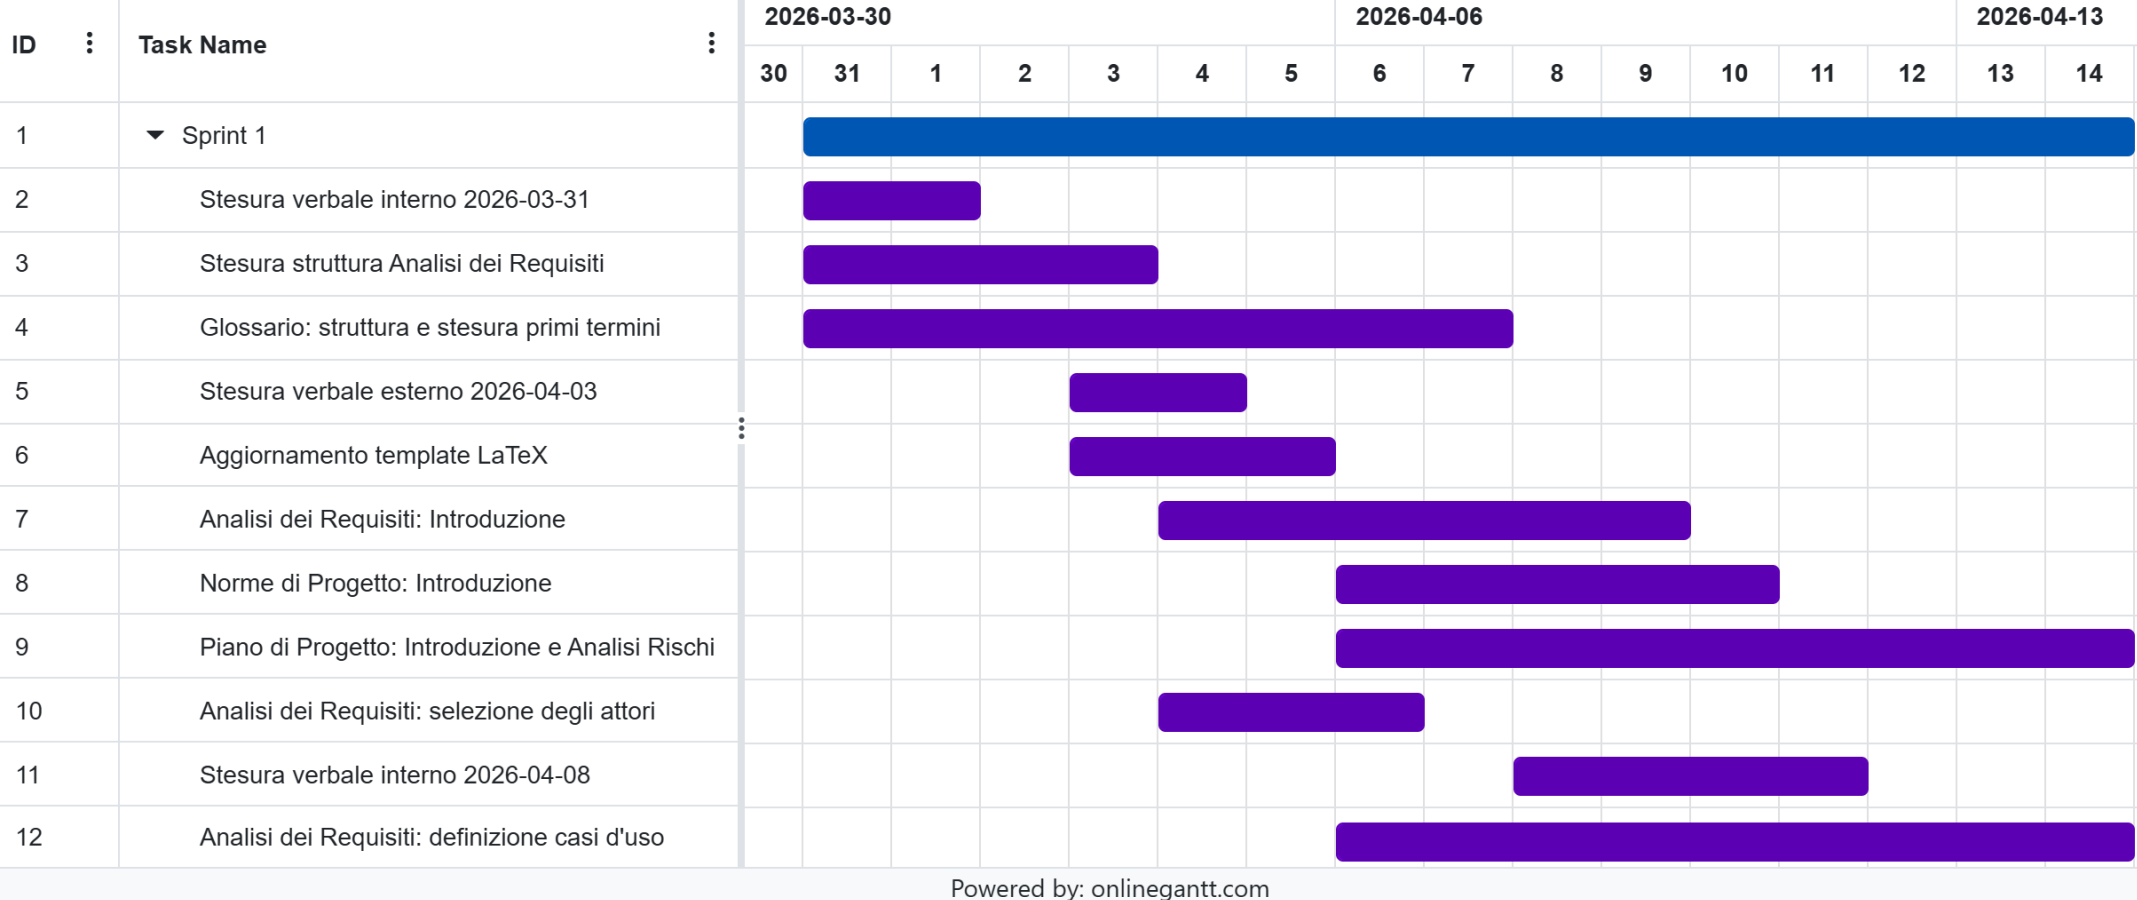
\includegraphics[width=\textwidth]{assets/gantt-sprint-1.png}
    \caption{Diagramma di Gantt dello Sprint 1}
    \label{fig:gantt-sprint1}
\end{figure}

\subsection{Sprint \#2: da 2026-04-14 a 2026-04-27}

\subsubsection{Obiettivi}

Durante il secondo sprint, il team prevede di consolidare e aggiornare la documentazione prodotta nello sprint\textsubscript{G} precedente, con particolare attenzione all'avanzamento dell'\textit{Analisi dei Requisiti}. L'obiettivo principale è passare dalla fase preliminare di studio e modellazione alla stesura più formale dei casi d'uso\textsubscript{G}, mantenendo allineati il \textit{Piano di Progetto}, le \textit{Norme di Progetto}, il \textit{Glossario} e l'\textit{Analisi dei Requisiti}.

Nello specifico, il team si impegnerà a:
\begin{itemize}
    \item proseguire la stesura del documento \textit{Analisi dei Requisiti}, avviando la descrizione formale dei casi d'uso\textsubscript{G} precedentemente studiati e modellati;

    \item completare la prima versione delle \textit{Norme di Progetto}, così da fornire al gruppo una base normativa condivisa per la gestione del lavoro, della documentazione e degli strumenti utilizzati;

    \item completare, all'interno del \textit{Piano di Progetto}, la sezione relativa all'analisi e alla gestione dei rischi e redigere il consuntivo e la retrospettiva dello Sprint\textsubscript{G} \#1, analizzando gli scostamenti rispetto al preventivo e individuando eventuali azioni correttive;

    \item aggiornare il \textit{Glossario} con i termini tecnici emersi durante la stesura della documentazione e durante le attività di analisi;

    \item avviare un'attività di brainstorming per il design preliminare UX/UI\textsubscript{G}, in vista della preparazione del mock-up\textsubscript{G} previsto per lo Sprint\textsubscript{G} \#3;

    \item redigere i verbali interni ed esterni relativi agli incontri svolti durante lo sprint\textsubscript{G}.
\end{itemize}

\subsection{Sprint \#3: da 2026-04-28 a 2026-05-11}

\subsubsection{Obiettivi}
Durante il terzo sprint\textsubscript{G}, il team prevede di concentrare le attività sul completamento dell'\textit{Analisi dei Requisiti} e sull'avvio delle prime attività progettuali legate al prodotto software. 

In questo sprint\textsubscript{G} viene inoltre introdotto il ruolo di Progettista, principalmente per la realizzazione del mock-up\textsubscript{G} dell'interfaccia utente e per le prime attività di raccordo tra requisiti, esperienza utente e futura implementazione del prodotto.

Nello specifico, il team si impegnerà a:
\begin{itemize}
    \item completare l'\textit{Analisi dei Requisiti}, realizzando i diagrammi UML\textsubscript{G} relativi ai casi d'uso\textsubscript{G};

    \item organizzare un incontro con la Proponente\textsubscript{G} per discutere i casi d'uso individuati, chiarire eventuali ambiguità e ottenere un riscontro prima di procedere con le fasi successive del progetto;

    \item avviare la realizzazione del mock-up\textsubscript{G} dell'interfaccia utente, definendo una prima rappresentazione grafica delle principali schermate e dei flussi di interazione dell'applicazione;

    \item svolgere uno studio iniziale delle tecnologie da adottare nello sviluppo del prodotto software, valutando quali strumenti risultino più adeguati per la realizzazione della web app\textsubscript{G};

    \item proseguire l'aggiornamento dei documenti di progetto, in particolare \textit{Piano di Progetto}, \textit{Norme di Progetto}, \textit{Glossario} e \textit{Analisi dei Requisiti};

    \item sviluppare uno script\textsubscript{G} per automatizzare la gestione dei termini del \textit{Glossario}, riducendo il lavoro manuale necessario per inserire nei documenti il riferimento ai termini glossarizzati;
    \item redigere i verbali interni ed esterni relativi agli incontri svolti durante lo sprintG.
\end{itemize}


\section{Preventivo}
Il preventivo viene elaborato considerando il costo orario associato a ciascun ruolo, il budget complessivo previsto e le attività pianificate per il periodo di riferimento. Per ogni sprint\textsubscript{G} vengono quindi riportati:

\begin{itemize}
    \item un preventivo delle ore previste, organizzato in forma tabellare;
    \item un preventivo dei costi stimati, anch'esso presentato in forma tabellare;
    \item un areogramma che rappresenta la distribuzione delle ore tra i diversi ruoli di progetto.
\end{itemize}

Il carico di lavoro complessivo previsto per ciascun componente del gruppo è pari a 92 ore, distribuite tra i diversi ruoli di progetto, per un totale di 646 ore produttive. La ripartizione delle mansioni viene gestita tramite un meccanismo di rotazione, con l'obiettivo di garantire a ogni membro del team la possibilità di ricoprire ruoli differenti e acquisire una visione più completa del processo di sviluppo.

Per rendere le tabelle più leggibili e compatte, i ruoli di progetto vengono indicati mediante le seguenti abbreviazioni\textsubscript{G}:

\begin{itemize}
    \item \textbf{Re}: Responsabile di progetto;
    \item \textbf{Am}: Amministratore;
    \item \textbf{An}: Analista;
    \item \textbf{Pt}: Progettista;
    \item \textbf{Pr}: Programmatore;
    \item \textbf{Ve}: Verificatore.
\end{itemize}

\subsection{Sprint \#1: da 2026-03-31 a 2026-04-13}
Di seguito è riportata la distribuzione delle ore per ciascun membro del team,
accumulate in totali per persona e per ruolo:

\begin{table}[H]
    \centering
    \renewcommand{\arraystretch}{1.4}
    \begin{tabular}{|l|c|c|c|c|c|c|c|}
        \hline
        \rowcolor{bluBitless!15}
        \textbf{Membro} & \textbf{Re} & \textbf{Am} & \textbf{An} & \textbf{Pt} & \textbf{Pr} & \textbf{Ve} & \textbf{Totale per persona} \\
        \hline
        L. Battistella & - & - & 7 & - & - & - & 7 \\ \hline
        E. De Piccoli & - & 5 & - & - & - & - & 5 \\ \hline
        D. Facco & - & - & 7 & - & - & - & 7 \\ \hline
        A. Marini & - & - & 7 & - & - & - & 7 \\ \hline
        A. Menegaldo & - & - & - & - & - & 8 & 8 \\ \hline
        S. Vendramin & 5 & - & - & - & - & - & 5 \\ \hline
        S. Zecchinato & - & - & 7 & - & - & - & 7 \\ \hline
        \rowcolor{bluBitless!8}
        \textbf{Totale per ruolo} & \textbf{5} & \textbf{5} & \textbf{28} & \textbf{-} & \textbf{-} & \textbf{8} & \textbf{46} \\
        \hline
    \end{tabular}
    \caption{\textit{Preventivo orario Sprint \#1}}
\end{table}

\begin{figure}[H]
\centering

\begin{tikzpicture}[scale=0.85]

% Colori pastello
\definecolor{colResp}{HTML}{BFE8DD}
\definecolor{colAmm}{HTML}{FFD0B5}
\definecolor{colAn}{HTML}{E4C9F5}
\definecolor{colVe}{HTML}{CDEBFF}
\definecolor{lineGray}{HTML}{8A8A8A}

% Raggio dell'areogramma
\def\r{3.2}

% Titolo
\node[font=\Large\bfseries] at (0,4.25) {Distribuzione ore per ruolo};

% Settori
% Totale = 46
% Re = 5 -> 10,9%
% Am = 5 -> 10,9%
% An = 28 -> 60,9%
% Ve = 8 -> 17,4%

\path[fill=colResp, draw=white, line width=1.5pt]
(0,0) -- (90:\r) arc[start angle=90,end angle=50.87,radius=\r] -- cycle;

\path[fill=colAmm, draw=white, line width=1.5pt]
(0,0) -- (50.87:\r) arc[start angle=50.87,end angle=11.74,radius=\r] -- cycle;

\path[fill=colAn, draw=white, line width=1.5pt]
(0,0) -- (11.74:\r) arc[start angle=11.74,end angle=-207.39,radius=\r] -- cycle;

\path[fill=colVe, draw=white, line width=1.5pt]
(0,0) -- (-207.39:\r) arc[start angle=-207.39,end angle=-270,radius=\r] -- cycle;

% Percentuali interne più piccole
\node[font=\normalsize\bfseries] at (70:1.75) {10,9\%};
\node[font=\normalsize\bfseries] at (31:1.85) {10,9\%};
\node[font=\normalsize\bfseries] at (-98:1.55) {60,9\%};
\node[font=\normalsize\bfseries] at (131:1.85) {17,4\%};

% Linee ed etichette esterne - Responsabile
\fill[lineGray] (1.25,2.75) circle (1.7pt);
\draw[lineGray, line width=0.7pt] (1.25,2.75) -- (3.65,2.75) -- (5.5,2.75);
\node[anchor=south east, font=\normalsize\bfseries] at (5.5,2.82) {Responsabile};
\node[anchor=north east, font=\small\bfseries, text=lineGray] at (5.5,2.60) {5 ore};

% Linee ed etichette esterne - Amministratore
\fill[lineGray] (2.85,1.05) circle (1.7pt);
\draw[lineGray, line width=0.7pt] (2.85,1.05) -- (4.0,1.05) -- (5.55,1.05);
\node[anchor=south east, font=\normalsize\bfseries] at (5.55,1.12) {Amministratore};
\node[anchor=north east, font=\small\bfseries, text=lineGray] at (5.55,0.90) {5 ore};

% Linee ed etichette esterne - Analista
\fill[lineGray] (-1.35,-2.65) circle (1.7pt);
\draw[lineGray, line width=0.7pt] (-1.35,-2.65) -- (-3.65,-2.65) -- (-5.45,-2.65);
\node[anchor=south west, font=\normalsize\bfseries] at (-5.45,-2.58) {Analista};
\node[anchor=north west, font=\small\bfseries, text=lineGray] at (-5.45,-2.80) {28 ore};

% Linee ed etichette esterne - Verificatore
\fill[lineGray] (-2.15,2.35) circle (1.7pt);
\draw[lineGray, line width=0.7pt] (-2.15,2.35) -- (-3.9,2.35) -- (-5.45,2.35);
\node[anchor=south west, font=\normalsize\bfseries] at (-5.45,2.42) {Verificatore};
\node[anchor=north west, font=\small\bfseries, text=lineGray] at (-5.45,2.20) {8 ore};

\end{tikzpicture}

\caption{Areogramma del preventivo orario nello Sprint \#1}
\label{fig:preventivo-sprint1}
\end{figure}

Di seguito è riportato il preventivo economico del primo sprint$G$:

\begin{table}[H]
    \centering
    \renewcommand{\arraystretch}{1.4}
    \begin{tabular}{|l|c|c|}
        \hline
        \rowcolor{bluBitless!15}
        \textbf{Ruolo} & \textbf{Ore per ruolo} & \textbf{Costo (in €)} \\
        \hline
        Responsabile di progetto & 5 & 150,00 \\ \hline
        Amministratore & 5 & 100,00 \\ \hline  
        Analista & 28 & 700,00 \\ \hline
        Progettista & 0 & 0,00 \\ \hline
        Programmatore & 0 & 0,00 \\ \hline
        Verificatore & 8 & 120,00 \\ \hline
        \rowcolor{bluBitless!8}
        \textbf{Totale} & \textbf{46} & \textbf{1.070,00} \\ \hline
    \end{tabular}
    \caption{\textit{Preventivo economico dello Sprint \#1}}
\end{table}

\subsection{Sprint \#2: da 2026-03-14 a 2026-04-27}
Di seguito è riportata la distribuzione delle ore per ciascun membro del team,
accumulate in totali per persona e per ruolo:
\begin{table}[H]
    \centering
    \renewcommand{\arraystretch}{1.4}
    \begin{tabular}{|l|c|c|c|c|c|c|c|}
        \hline
        \rowcolor{bluBitless!15}
        \textbf{Membro} & \textbf{Re} & \textbf{Am} & \textbf{An} & \textbf{Pt} & \textbf{Pr} & \textbf{Ve} & \textbf{Totale per persona} \\
        \hline
        L. Battistella & 6 & - & - & - & - & - & 6 \\ \hline
        E. De Piccoli & - & - & - & - & - & 6 & 6 \\ \hline
        D. Facco & - & - & - & - & - & 6 & 6 \\ \hline
        A. Marini & - & 7 & - & - & - & - & 7 \\ \hline
        A. Menegaldo & - & - & 6 & - & - & - & 6 \\ \hline
        S. Vendramin & - & - & 6 & - & - & - & 6 \\ \hline
        S. Zecchinato & - & - & 6 & - & - & - & 6 \\ \hline
        \rowcolor{bluBitless!8}
        \textbf{Totale per ruolo} & \textbf{6} & \textbf{7} & \textbf{18} & \textbf{-} & \textbf{-} & \textbf{12} & \textbf{43} \\
        \hline
    \end{tabular}
    \caption{\textit{Preventivo orario Sprint \#2}}
\end{table}

\begin{figure}[H]
\centering

\begin{tikzpicture}[scale=0.85]

% Colori pastello
\definecolor{colResp}{HTML}{BFE8DD}
\definecolor{colAmm}{HTML}{FFD0B5}
\definecolor{colAn}{HTML}{E4C9F5}
\definecolor{colVe}{HTML}{CDEBFF}
\definecolor{lineGray}{HTML}{8A8A8A}

% Raggio dell'areogramma
\def\r{3.2}

% Titolo
\node[font=\Large\bfseries] at (0,4.25) {Distribuzione ore per ruolo};

% Totale = 43
% Re = 6  -> 14,0%
% Am = 7  -> 16,3%
% An = 18 -> 41,9%
% Ve = 12 -> 27,9%

% Settori
\path[fill=colResp, draw=white, line width=1.5pt]
(0,0) -- (90:\r) arc[start angle=90,end angle=39.77,radius=\r] -- cycle;

\path[fill=colAmm, draw=white, line width=1.5pt]
(0,0) -- (39.77:\r) arc[start angle=39.77,end angle=-18.84,radius=\r] -- cycle;

\path[fill=colAn, draw=white, line width=1.5pt]
(0,0) -- (-18.84:\r) arc[start angle=-18.84,end angle=-169.53,radius=\r] -- cycle;

\path[fill=colVe, draw=white, line width=1.5pt]
(0,0) -- (-169.53:\r) arc[start angle=-169.53,end angle=-270,radius=\r] -- cycle;

% Percentuali interne
\node[font=\normalsize\bfseries] at (65:1.75) {14,0\%};
\node[font=\normalsize\bfseries] at (10:1.85) {16,3\%};
\node[font=\normalsize\bfseries] at (-95:1.55) {41,9\%};
\node[font=\normalsize\bfseries] at (140:1.85) {27,9\%};

% Linee ed etichette esterne - Responsabile
\fill[lineGray] (1.60,2.50) circle (1.7pt);
\draw[lineGray, line width=0.7pt] (1.60,2.50) -- (3.65,2.50) -- (5.5,2.50);
\node[anchor=south east, font=\normalsize\bfseries] at (5.5,2.57) {Responsabile};
\node[anchor=north east, font=\small\bfseries, text=lineGray] at (5.5,2.35) {6 ore};

% Linee ed etichette esterne - Amministratore
\fill[lineGray] (3.00,0.35) circle (1.7pt);
\draw[lineGray, line width=0.7pt] (3.00,0.35) -- (4.0,0.35) -- (5.55,0.35);
\node[anchor=south east, font=\normalsize\bfseries] at (5.55,0.42) {Amministratore};
\node[anchor=north east, font=\small\bfseries, text=lineGray] at (5.55,0.20) {7 ore};

% Linee ed etichette esterne - Analista
\fill[lineGray] (-0.70,-3.00) circle (1.7pt);
\draw[lineGray, line width=0.7pt] (-0.70,-3.00) -- (-3.65,-3.00) -- (-5.45,-3.00);
\node[anchor=south west, font=\normalsize\bfseries] at (-5.45,-2.93) {Analista};
\node[anchor=north west, font=\small\bfseries, text=lineGray] at (-5.45,-3.15) {18 ore};

% Linee ed etichette esterne - Verificatore
\fill[lineGray] (-2.20,2.30) circle (1.7pt);
\draw[lineGray, line width=0.7pt] (-2.20,2.30) -- (-3.9,2.30) -- (-5.45,2.30);
\node[anchor=south west, font=\normalsize\bfseries] at (-5.45,2.37) {Verificatore};
\node[anchor=north west, font=\small\bfseries, text=lineGray] at (-5.45,2.15) {12 ore};

\end{tikzpicture}

\caption{Areogramma della distribuzione delle ore per ruolo nello Sprint \#2}
\label{fig:preventivo-sprint2}
\end{figure}

Di seguito è riportato il preventivo economico del secondo sprint\textsubscript{G}:

\begin{table}[H]
    \centering
    \renewcommand{\arraystretch}{1.4}
    \begin{tabular}{|l|c|c|}
        \hline
        \rowcolor{bluBitless!15}
        \textbf{Ruolo} & \textbf{Ore per ruolo} & \textbf{Costo (in €)} \\
        \hline
        Responsabile di progetto & 6 & 180,00 \\ \hline
        Amministratore & 7 & 140,00 \\ \hline
        Analista & 18 & 450,00 \\ \hline
        Progettista & 0 & 0,00 \\ \hline
        Programmatore & 0 & 0,00 \\ \hline
        Verificatore & 12 & 180,00 \\ \hline
        \rowcolor{bluBitless!8}
        \textbf{Totale} & \textbf{43} & \textbf{950,00} \\ \hline
    \end{tabular}
    \caption{\textit{Preventivo economico dello Sprint \#2}}
\end{table}


\subsection{Sprint \#3: da 2026-04-28 a 2026-05-11}
Di seguito è riportata la distribuzione delle ore per ciascun membro del team,
accumulate in totali per persona e per ruolo:

\begin{table}[H]
    \centering
    \renewcommand{\arraystretch}{1.4}
    \begin{tabular}{|l|c|c|c|c|c|c|c|}
        \hline
        \rowcolor{bluBitless!15}
        \textbf{Membro} & \textbf{Re} & \textbf{Am} & \textbf{An} & \textbf{Pt} & \textbf{Pr} & \textbf{Ve} & \textbf{Totale per persona} \\
        \hline
        L. Battistella & - & 7 & - & - & - & - & 7 \\ \hline
        E. De Piccoli & - & - & 7 & - & - & - & 7 \\ \hline
        D. Facco & - & - & - & 7 & - & - & 7 \\ \hline
        A. Marini & 4 & - & 3 & - & - & - & 7 \\ \hline
        A. Menegaldo & - & - & - & - & - & 6 & 6 \\ \hline
        S. Vendramin & - & - & - & 6 & - & - & 6 \\ \hline
        S. Zecchinato & - & - & - & - & - & 7 & 7 \\ \hline
        \rowcolor{bluBitless!8}
        \textbf{Totale per ruolo} & \textbf{4} & \textbf{7} & \textbf{10} & \textbf{13} & \textbf{-} & \textbf{13} & \textbf{47} \\
        \hline
    \end{tabular}
    \caption{\textit{Preventivo orario Sprint \#3}}
\end{table}

\begin{figure}[H]
\centering

\begin{tikzpicture}[scale=0.85]

% Colori pastello
\definecolor{colResp}{HTML}{BFD7EA}
\definecolor{colAmm}{HTML}{F7C8C8}
\definecolor{colAn}{HTML}{D8C4F2}
\definecolor{colPt}{HTML}{FFE5B4}
\definecolor{colVe}{HTML}{CDECCF}
\definecolor{lineGray}{HTML}{8A8A8A}

% Raggio dell'areogramma
\def\r{3.2}

% Titolo
\node[font=\Large\bfseries] at (0,4.25) {Distribuzione ore per ruolo};

% Totale = 47
% Re = 4  -> 8,5%
% Am = 7  -> 14,9%
% An = 10 -> 21,3%
% Pt = 13 -> 27,7%
% Ve = 13 -> 27,7%

% Settori
\path[fill=colResp, draw=white, line width=1.5pt]
(0,0) -- (90:\r) arc[start angle=90,end angle=59.36,radius=\r] -- cycle;

\path[fill=colAmm, draw=white, line width=1.5pt]
(0,0) -- (59.36:\r) arc[start angle=59.36,end angle=5.74,radius=\r] -- cycle;

\path[fill=colAn, draw=white, line width=1.5pt]
(0,0) -- (5.74:\r) arc[start angle=5.74,end angle=-70.85,radius=\r] -- cycle;

\path[fill=colPt, draw=white, line width=1.5pt]
(0,0) -- (-70.85:\r) arc[start angle=-70.85,end angle=-170.43,radius=\r] -- cycle;

\path[fill=colVe, draw=white, line width=1.5pt]
(0,0) -- (-170.43:\r) arc[start angle=-170.43,end angle=-270,radius=\r] -- cycle;

% Percentuali interne
\node[font=\small\bfseries] at (75:1.65) {8,5\%};
\node[font=\small\bfseries] at (32:1.75) {14,9\%};
\node[font=\small\bfseries] at (-32:1.75) {21,3\%};
\node[font=\small\bfseries] at (-120:1.75) {27,7\%};
\node[font=\small\bfseries] at (140:1.75) {27,7\%};

% Responsabile
\fill[lineGray] (0.95,2.90) circle (1.7pt);
\draw[lineGray, line width=0.7pt] (0.95,2.90) -- (3.65,2.90) -- (5.5,2.90);
\node[anchor=south east, font=\normalsize\bfseries] at (5.5,2.97) {Responsabile};
\node[anchor=north east, font=\small\bfseries, text=lineGray] at (5.5,2.75) {4 ore};

% Amministratore
\fill[lineGray] (2.75,1.25) circle (1.7pt);
\draw[lineGray, line width=0.7pt] (2.75,1.25) -- (4.0,1.25) -- (5.55,1.25);
\node[anchor=south east, font=\normalsize\bfseries] at (5.55,1.32) {Amministratore};
\node[anchor=north east, font=\small\bfseries, text=lineGray] at (5.55,1.10) {7 ore};

% Analista
\fill[lineGray] (2.65,-1.25) circle (1.7pt);
\draw[lineGray, line width=0.7pt] (2.65,-1.25) -- (4.0,-1.25) -- (5.55,-1.25);
\node[anchor=south east, font=\normalsize\bfseries] at (5.55,-1.18) {Analista};
\node[anchor=north east, font=\small\bfseries, text=lineGray] at (5.55,-1.40) {10 ore};

% Progettista
\fill[lineGray] (-1.85,-2.45) circle (1.7pt);
\draw[lineGray, line width=0.7pt] (-1.85,-2.45) -- (-3.75,-2.45) -- (-5.45,-2.45);
\node[anchor=south west, font=\normalsize\bfseries] at (-5.45,-2.38) {Progettista};
\node[anchor=north west, font=\small\bfseries, text=lineGray] at (-5.45,-2.60) {13 ore};

% Verificatore
\fill[lineGray] (-2.30,2.15) circle (1.7pt);
\draw[lineGray, line width=0.7pt] (-2.30,2.15) -- (-3.9,2.15) -- (-5.45,2.15);
\node[anchor=south west, font=\normalsize\bfseries] at (-5.45,2.22) {Verificatore};
\node[anchor=north west, font=\small\bfseries, text=lineGray] at (-5.45,2.00) {13 ore};

\end{tikzpicture}

\caption{Areogramma del preventivo orario nello Sprint \#3}
\label{fig:preventivo-sprint3}
\end{figure}

Di seguito è riportato il preventivo economico del terzo sprint\textsubscript{G}:

\begin{table}[H]
    \centering
    \renewcommand{\arraystretch}{1.4}
    \begin{tabular}{|l|c|c|}
        \hline
        \rowcolor{bluBitless!15}
        \textbf{Ruolo} & \textbf{Ore per ruolo} & \textbf{Costo (in €)} \\
        \hline
        Responsabile di progetto & 4 & 120,00 \\ \hline
        Amministratore & 7 & 140,00 \\ \hline
        Analista & 10 & 250,00 \\ \hline
        Progettista & 13 & 325,00 \\ \hline
        Programmatore & 0 & 0,00 \\ \hline
        Verificatore & 13 & 195,00 \\ \hline
        \rowcolor{bluBitless!8}
        \textbf{Totale} & \textbf{47} & \textbf{1.030,00} \\ \hline
    \end{tabular}
    \caption{\textit{Preventivo economico dello Sprint \#3}}
\end{table}




\section{Consuntivo}
Il consuntivo rappresenta la stima aggiornata delle ore e dei costi effettivamente impiegati durante lo sprint\textsubscript{G}, confrontati con le previsioni iniziali. Questa fase è fondamentale per valutare l'andamento del progetto, identificare eventuali scostamenti rispetto alla pianificazione e aggiornare il preventivo a finire.
Il consuntivo viene elaborato al termine di ogni sprint\textsubscript{G},tenendo conto delle ore rendicontate dai membri del gruppo, delle attività completate e di eventuali difficoltà incontrate durante l'iterazione. Inoltre, vengono analizzati i motivi di eventuali scostamenti rispetto al preventivo iniziale, così da individuare azioni correttive da applicare negli sprint\textsubscript{G} successivi.

\subsection{Sprint \#1: da 2026-03-31 a 2026-04-14}

Di seguito è riportata la distribuzione delle ore per ciascun membro del team,
accumulate in totali per persona e per ruolo:
\begin{table}[H]
    \centering
    \renewcommand{\arraystretch}{1.4}
    \begin{tabular}{|l|c|c|c|c|c|c|c|}
        \hline
        \rowcolor{bluBitless!15}
        \textbf{Membro} & \textbf{Re} & \textbf{Am} & \textbf{An} & \textbf{Pt} & \textbf{Pr} & \textbf{Ve} & \textbf{Totale per persona} \\
        \hline
        L. Battistella & - & - & 6 & - & - & - & 6 \\ \hline
        E. De Piccoli & - & 5 & - & - & - & - & 5 \\ \hline
        D. Facco & - & - & 6 & - & - & - & 6 \\ \hline
        A. Marini & - & - & 6 & - & - & - & 6 \\ \hline
        A. Menegaldo & - & - & - & - & - & 8 & 8 \\ \hline
        S. Vendramin & 7 & - & - & - & - & - & 7 \\ \hline
        S. Zecchinato & - & - & 6 & - & - & - & 6 \\ \hline
        \rowcolor{bluBitless!8}
        \textbf{Totale per ruolo} & \textbf{7} & \textbf{5} & \textbf{24} & \textbf{-} & \textbf{-} & \textbf{8} & \textbf{44} \\
        \hline
    \end{tabular}
    \caption{\textit{Consuntivo orario Sprint \#1}}
\end{table}

\begin{figure}[H]
\centering

\begin{tikzpicture}[scale=0.85]

% Colori pastello
\definecolor{colResp}{HTML}{BFD7EA}
\definecolor{colAmm}{HTML}{F7C8C8}
\definecolor{colAn}{HTML}{D8C4F2}
\definecolor{colVe}{HTML}{CDECCF}
\definecolor{lineGray}{HTML}{8A8A8A}

% Raggio dell'areogramma
\def\r{3.2}

% Titolo
\node[font=\Large\bfseries] at (0,4.25) {Distribuzione ore per ruolo};

% Totale = 44
% Re = 7  -> 15,9%
% Am = 5  -> 11,4%
% An = 24 -> 54,5%
% Ve = 8  -> 18,2%

% Settori
\path[fill=colResp, draw=white, line width=1.5pt]
(0,0) -- (90:\r) arc[start angle=90,end angle=32.73,radius=\r] -- cycle;

\path[fill=colAmm, draw=white, line width=1.5pt]
(0,0) -- (32.73:\r) arc[start angle=32.73,end angle=-8.18,radius=\r] -- cycle;

\path[fill=colAn, draw=white, line width=1.5pt]
(0,0) -- (-8.18:\r) arc[start angle=-8.18,end angle=-204.55,radius=\r] -- cycle;

\path[fill=colVe, draw=white, line width=1.5pt]
(0,0) -- (-204.55:\r) arc[start angle=-204.55,end angle=-270,radius=\r] -- cycle;

% Percentuali interne
\node[font=\normalsize\bfseries] at (61:1.75) {15,9\%};
\node[font=\normalsize\bfseries] at (8:1.45) {11,4\%};
\node[font=\normalsize\bfseries] at (-106:1.55) {54,5\%};
\node[font=\normalsize\bfseries] at (123:1.85) {18,2\%};

% Linee ed etichette esterne - Responsabile
\fill[lineGray] (1.65,2.50) circle (1.7pt);
\draw[lineGray, line width=0.7pt] (1.65,2.50) -- (3.65,2.50) -- (5.5,2.50);
\node[anchor=south east, font=\normalsize\bfseries] at (5.5,2.57) {Responsabile};
\node[anchor=north east, font=\small\bfseries, text=lineGray] at (5.5,2.35) {7 ore};

% Linee ed etichette esterne - Amministratore
\fill[lineGray] (3.00,0.35) circle (1.7pt);
\draw[lineGray, line width=0.7pt] (3.00,0.35) -- (4.35,0.35) -- (5.95,0.35);
\node[anchor=south east, font=\normalsize\bfseries] at (5.95,0.42) {Amministratore};
\node[anchor=north east, font=\small\bfseries, text=lineGray] at (5.95,0.20) {5 ore};
% Linee ed etichette esterne - Analista
\fill[lineGray] (-1.10,-2.85) circle (1.7pt);
\draw[lineGray, line width=0.7pt] (-1.10,-2.85) -- (-3.65,-2.85) -- (-5.45,-2.85);
\node[anchor=south west, font=\normalsize\bfseries] at (-5.45,-2.78) {Analista};
\node[anchor=north west, font=\small\bfseries, text=lineGray] at (-5.45,-3.00) {24 ore};

% Linee ed etichette esterne - Verificatore
\fill[lineGray] (-2.15,2.35) circle (1.7pt);
\draw[lineGray, line width=0.7pt] (-2.15,2.35) -- (-3.9,2.35) -- (-5.45,2.35);
\node[anchor=south west, font=\normalsize\bfseries] at (-5.45,2.42) {Verificatore};
\node[anchor=north west, font=\small\bfseries, text=lineGray] at (-5.45,2.20) {8 ore};
\end{tikzpicture}
\caption{Areogramma della distribuzione delle ore consuntivate per ruolo nello Sprint \#1}
\label{fig:consuntivo-sprint1}
\end{figure}

Di seguito è riportato il consuntivo economico del primo sprintG: 
\begin{table}[H]
    \centering
    \renewcommand{\arraystretch}{1.4}
    \begin{tabular}{|l|c|c|c|c|}
        \hline
        \rowcolor{bluBitless!15}
        \textbf{Ruolo} & 
        \textbf{\shortstack{Ore per\\ruolo}} & 
        \textbf{\shortstack{Delta ore\\preventivo-\\consuntivo}} & 
        \textbf{Costo (in €)} & 
        \textbf{\shortstack{Delta costo\\preventivo-\\consuntivo(in €)}} \\
        \hline

        Responsabile di progetto & 7 & -2 & 210,00 & -60,00 \\ \hline
        Amministratore & 5 & 0 & 100,00 & 0,00 \\ \hline
        Analista & 24 & +4 & 600,00 & +100,00 \\ \hline
        Progettista & 0 & 0 & 0,00 & 0,00 \\ \hline
        Programmatore & 0 & 0 & 0,00 & 0,00 \\ \hline
        Verificatore & 8 & 0 & 120,00 & 0,00 \\ \hline

        \rowcolor{bluBitless!8}
        \textbf{Totale} & \textbf{44} & \textbf{+2} & \textbf{1.030,00} & \textbf{+40,00} \\ \hline

        Sprint pregressi & 0 & / & 0,00 & / \\ \hline
        Restante & 600 & / & 11.830,00 & / \\ \hline
    \end{tabular}
    \caption{\textit{Consuntivo economico Sprint \#1}}
\end{table}

Di seguito sono riportate le ore rimanenti per la coppia risorsa-ruolo:

\begin{table}[H]
    \centering
    \renewcommand{\arraystretch}{1.4}
    \begin{tabular}{|l|c|c|c|c|c|c|c|}
        \hline
        \rowcolor{bluBitless!15}
        \textbf{Membro del team} & \textbf{Re} & \textbf{Am} & \textbf{An} & \textbf{Pt} & \textbf{Pr} & \textbf{Ve} & \textbf{Totale per persona} \\
        \hline
        L. Battistella & 7 & 9 & 3 & 22 & 22 & 23 & 86 \\ \hline
        E. De Piccoli & 7 & 4 & 9 & 22 & 22 & 23 & 87 \\ \hline
        D. Facco & 7 & 8 & 3 & 22 & 23 & 23 & 86 \\ \hline
        A. Marini & 7 & 8 & 3 & 22 & 23 & 23 & 86 \\ \hline
        A. Menegaldo & 7 & 8 & 9 & 23 & 22 & 15 & 84 \\ \hline
        S. Vendramin & 0 & 9 & 8 & 22 & 24 & 22 & 85 \\ \hline
        S. Zecchinato & 6 & 9 & 3 & 23 & 22 & 23 & 86 \\ \hline
        \rowcolor{bluBitless!8}
        \textbf{Totale per ruolo} & \textbf{41} & \textbf{55} & \textbf{38} & \textbf{156} & \textbf{158} & \textbf{152} & \textbf{600} \\
        \hline
    \end{tabular}
    \caption{\textit{Ore rimanenti per coppia risorsa-ruolo dopo lo Sprint \#1}}
\end{table}

\subsubsection{Revisione delle attività} 
Durante lo Sprint\textsubscript{G} \#1 il team ha svolto attività principalmente orientate alla definizione delle basi documentali e organizzative del progetto.
Le attività principali svolte sono state:
\begin{itemize}
    \item inizio dell'\textit{Analisi dei Requisiti}, con particolare attenzione a:
    \begin{itemize}
        \item studio preliminare della struttura dei casi d'uso\textsubscript{G};
        \item individuazione degli attori principali del sistema;
        \item definizione dei primi casi d'uso\textsubscript{G}; 
    \end{itemize} 
    \item avvio della stesura del \textit{Piano di Progetto}, comprendendo l'avvio dell'analisi dei rischi tecnologici e organizzativi;
    \item avvio della stesura delle \textit{Norme di Progetto};
    \item miglioramento del Way of Working\textsubscript{G}, con l'obiettivo di definire modalità comuni per la gestione del lavoro;      
    \item pianificazione e preventivazione delle attività relative allo Sprint\textsubscript{G} \#2;
    \item inserimento nel \textit{Glossario} dei primi termini tecnici utilizzati durante la candidatura e nelle prime attività progettuali;
    \item redazione dei verbali interni ed esterni.
\end{itemize}

\subsubsection{Gestione dei rischi}
\begin{itemize}
    \item \textbf{Rischi attesi e occorsi:}

    \begin{itemize}
        \item \textbf{RO-5 - Scarsa esperienza nel lavoro di gruppo}

        \begin{itemize}
            \item \textbf{Esito mitigazione:} le misure di mitigazione previste si sono rivelate solo parzialmente efficaci durante il primo sprint\textsubscript{G}. Il gruppo si trovava infatti nella fase iniziale del progetto e non aveva ancora consolidato un metodo di lavoro comune. Le \textit{Norme di Progetto} erano ancora in fase di stesura, quindi non fornivano ancora una guida completa e stabile per la gestione operativa delle attività.

            Alcuni task\textsubscript{G} sono stati assegnati in modo troppo generale, senza una suddivisione sufficientemente precisa delle attività da svolgere. Questo ha generato qualche difficoltà nel comprendere con chiarezza chi dovesse occuparsi di determinate parti del lavoro e quale risultato fosse atteso da ciascun membro.

            \item \textbf{Impatto:} l'impatto complessivo è stato contenuto, poiché il rischio si è manifestato in una fase ancora iniziale del progetto, quando la quantità di documentazione da gestire era limitata. Tuttavia, l'evento ha evidenziato la necessità di definire task\textsubscript{G} più specifici, responsabilità più chiare e momenti di confronto più frequenti tra i membri del gruppo.
        \end{itemize}

        \item \textbf{RO-6 - Scarsa esperienza nell'utilizzo degli strumenti di sviluppo}

        \begin{itemize}
            \item \textbf{Esito mitigazione:} il rischio si è manifestato principalmente nell'utilizzo non ancora uniforme degli strumenti di supporto allo sviluppo e alla gestione del progetto, in particolare GitHub\textsubscript{G}, issue\textsubscript{G}, milestone\textsubscript{G}, branch\textsubscript{G} e strumenti di project tracking\textsubscript{G}. 

            Le misure di mitigazione previste si sono rivelate parzialmente efficaci, poiché il team ha iniziato a prendere familiarità con tali strumenti durante lo sprint\textsubscript{G}, ma non disponeva ancora di procedure operative completamente definite. La mancanza iniziale di una lista puntuale delle attività da svolgere ha reso meno immediata la gestione delle issue\textsubscript{G} e l'assegnazione dei compiti ai singoli membri.

            \item \textbf{Impatto:} l'impatto non ha compromesso le scadenze dello sprint\textsubscript{G}, ma ha generato alcune inefficienze organizzative. In particolare, è stato necessario dedicare tempo alla comprensione degli strumenti e al loro utilizzo corretto, riducendo parzialmente le ore di produzione effettiva.
        \end{itemize}
    \end{itemize}
    \item \textbf{Rischi attesi ma non occorsi:}
    \begin{itemize}
        \item Nessuno.
    \end{itemize}
\end{itemize}

\subsubsection{Retrospettiva}
Dall'analisi dello Sprint\textsubscript{G} \#1 sono emersi alcuni scostamenti tra preventivo e consuntivo.

\begin{itemize}
    \item \textbf{Scostamento del ruolo Analista:}
    le ore consuntivate per il ruolo di Analista sono risultate inferiori rispetto a quelle preventivate. 
    Parte del tempo è stata infatti dedicata allo studio preliminare dei casi d'uso\textsubscript{G}, degli attori del sistema, della struttura dei diagrammi UML\textsubscript{G} e delle modalità corrette di documentazione. 
    Le ore preventivate consideravano soprattutto la produzione effettiva della documentazione, mentre nella pratica è stato necessario dedicare tempo anche alla fase di apprendimento.

    \item \textbf{Scostamento del ruolo Responsabile:}
    il ruolo di Responsabile ha richiesto 2 ore in più rispetto al preventivo. 
    Essendo il primo sprint\textsubscript{G}, il gruppo ha avuto bisogno di maggiore coordinamento per chiarire le attività da svolgere, le priorità, l'utilizzo degli strumenti di tracciamento e la suddivisione dei compiti tra i membri.

    \item \textbf{Problemi principali rilevati:}
    sono stati individuati alcuni problemi organizzativi, tra cui task\textsubscript{G} inizialmente troppo generici, mancanza di una lista puntuale delle attività da svolgere, uso non ancora uniforme degli strumenti di project tracking\textsubscript{G} e comunicazione interna non sempre sufficiente.
\end{itemize}

\subsubsection{Azioni correttive e miglioramenti previsti}
A partire dalle criticità emerse durante lo Sprint\textsubscript{G} \#1, il gruppo ha individuato alcune azioni correttive da applicare negli sprint\textsubscript{G} successivi.

\begin{itemize}
    \item definire task\textsubscript{G} più dettagliati, meno generici e facilmente verificabili;
    \item assegnare le attività in modo più chiaro, specificando responsabilità e risultati attesi per ciascun membro;
    \item migliorare la comunicazione interna, favorendo un confronto più costante sull'avanzamento delle attività;
    \item utilizzare in modo più sistematico GitHub\textsubscript{G} per il tracciamento dei task\textsubscript{G}, delle issue\textsubscript{G} e delle milestone\textsubscript{G};
    \item completare e applicare in modo più rigoroso quanto definito nelle \textit{Norme di Progetto}, così da rendere più stabile e uniforme il Way of Working\textsubscript{G}.
\end{itemize}

\subsection{Sprint \#2: da 2026-03-14 a 2026-04-27}
Di seguito è riportata la distribuzione delle ore per ciascun membro del team,
accumulate in totali per persona e per ruolo:

\begin{table}[H]
    \centering
    \renewcommand{\arraystretch}{1.4}
    \begin{tabular}{|l|c|c|c|c|c|c|c|}
        \hline
        \rowcolor{bluBitless!15}
        \textbf{Membro} & \textbf{Re} & \textbf{Am} & \textbf{An} & \textbf{Pt} & \textbf{Pr} & \textbf{Ve} & \textbf{Totale per persona} \\
        \hline
        L. Battistella & 5 & - & 2 & - & - & - & 7 \\ \hline
        E. De Piccoli & - & - & - & - & - & 6 & 6 \\ \hline
        D. Facco & - & - & - & - & - & 7 & 7 \\ \hline
        A. Marini & - & 7 & - & - & - & - & 7 \\ \hline
        A. Menegaldo & - & - & 6 & - & - & - & 6 \\ \hline
        S. Vendramin & - & - & 7 & - & - & - & 7 \\ \hline
        S. Zecchinato & - & - & 3 & - & - & 3 & 6 \\ \hline
        \rowcolor{bluBitless!8}
        \textbf{Totale per ruolo} & \textbf{5} & \textbf{7} & \textbf{18} & \textbf{-} & \textbf{-} & \textbf{16} & \textbf{46} \\
        \hline
    \end{tabular}
    \caption{\textit{Consuntivo orario Sprint \#2}}
\end{table}

\begin{figure}[H]
\centering

\begin{tikzpicture}[scale=0.85]

% Colori pastello
\definecolor{colResp}{HTML}{BFE8DD}
\definecolor{colAmm}{HTML}{FFD0B5}
\definecolor{colAn}{HTML}{E4C9F5}
\definecolor{colVe}{HTML}{CDEBFF}
\definecolor{lineGray}{HTML}{8A8A8A}

% Raggio dell'areogramma
\def\r{3.2}

% Titolo
\node[font=\Large\bfseries] at (0,4.25) {Distribuzione ore per ruolo};

% Totale = 46
% Re = 5  -> 10,9%
% Am = 7  -> 15,2%
% An = 18 -> 39,1%
% Ve = 16 -> 34,8%

% Settori
\path[fill=colResp, draw=white, line width=1.5pt]
(0,0) -- (90:\r) arc[start angle=90,end angle=50.87,radius=\r] -- cycle;

\path[fill=colAmm, draw=white, line width=1.5pt]
(0,0) -- (50.87:\r) arc[start angle=50.87,end angle=-3.91,radius=\r] -- cycle;

\path[fill=colAn, draw=white, line width=1.5pt]
(0,0) -- (-3.91:\r) arc[start angle=-3.91,end angle=-144.78,radius=\r] -- cycle;

\path[fill=colVe, draw=white, line width=1.5pt]
(0,0) -- (-144.78:\r) arc[start angle=-144.78,end angle=-270,radius=\r] -- cycle;

% Percentuali interne
\node[font=\normalsize\bfseries] at (70:1.75) {10,9\%};
\node[font=\normalsize\bfseries] at (24:1.85) {15,2\%};
\node[font=\normalsize\bfseries] at (-75:1.55) {39,1\%};
\node[font=\normalsize\bfseries] at (150:1.85) {34,8\%};

% Linee ed etichette esterne - Responsabile
\fill[lineGray] (1.25,2.75) circle (1.7pt);
\draw[lineGray, line width=0.7pt] (1.25,2.75) -- (3.65,2.75) -- (5.5,2.75);
\node[anchor=south east, font=\normalsize\bfseries] at (5.5,2.82) {Responsabile};
\node[anchor=north east, font=\small\bfseries, text=lineGray] at (5.5,2.60) {5 ore};

% Linee ed etichette esterne - Amministratore
\fill[lineGray] (2.95,0.95) circle (1.7pt);
\draw[lineGray, line width=0.7pt] (2.95,0.95) -- (4.0,0.95) -- (5.55,0.95);
\node[anchor=south east, font=\normalsize\bfseries] at (5.55,1.02) {Amministratore};
\node[anchor=north east, font=\small\bfseries, text=lineGray] at (5.55,0.80) {7 ore};

% Linee ed etichette esterne - Analista
\fill[lineGray] (-0.60,-3.00) circle (1.7pt);
\draw[lineGray, line width=0.7pt] (-0.60,-3.00) -- (-3.65,-3.00) -- (-5.45,-3.00);
\node[anchor=south west, font=\normalsize\bfseries] at (-5.45,-2.93) {Analista};
\node[anchor=north west, font=\small\bfseries, text=lineGray] at (-5.45,-3.15) {18 ore};

% Linee ed etichette esterne - Verificatore
\fill[lineGray] (-2.20,2.30) circle (1.7pt);
\draw[lineGray, line width=0.7pt] (-2.20,2.30) -- (-3.9,2.30) -- (-5.45,2.30);
\node[anchor=south west, font=\normalsize\bfseries] at (-5.45,2.37) {Verificatore};
\node[anchor=north west, font=\small\bfseries, text=lineGray] at (-5.45,2.15) {16 ore};

\end{tikzpicture}

\caption{Areogramma della distribuzione delle ore consuntivate per ruolo nello Sprint \#2}
\label{fig:consuntivo-sprint2}
\end{figure}

Di seguito è riportato il consuntivo economico del secondo sprint\textsubscript{G}:

\begin{table}[H]
    \centering
    \renewcommand{\arraystretch}{1.4}
    \begin{tabular}{|l|c|c|c|c|}
        \hline
        \rowcolor{bluBitless!15}
        \textbf{Ruolo} & 
        \textbf{\shortstack{Ore per\\ruolo}} & 
        \textbf{\shortstack{Delta ore\\preventivo-\\consuntivo}} & 
        \textbf{Costo (in €)} & 
        \textbf{\shortstack{Delta costo\\preventivo-\\consuntivo\\(in €)}} \\
        \hline

        Responsabile di progetto & 5 & +1 & 150,00 & +30,00 \\ \hline
        Amministratore & 7 & 0 & 140,00 & 0,00 \\ \hline
        Analista & 18 & 0 & 450,00 & 0,00 \\ \hline
        Progettista & 0 & 0 & 0,00 & 0,00 \\ \hline
        Programmatore & 0 & 0 & 0,00 & 0,00 \\ \hline
        Verificatore & 16 & -4 & 240,00 & -60,00 \\ \hline

        \rowcolor{bluBitless!8}
        \textbf{Totale} & \textbf{46} & \textbf{-3} & \textbf{980,00} & \textbf{-30,00} \\ \hline

        Sprint pregressi & 44 & / & 1.030,00 & / \\ \hline
        Restante & 554 & / & 10.850,00 & / \\ \hline
    \end{tabular}
    \caption{\textit{Consuntivo economico Sprint \#2}}
\end{table}

Di seguito sono riportate le ore rimanenti per la coppia risorsa-ruolo:

\begin{table}[H]
    \centering
    \renewcommand{\arraystretch}{1.4}
    \begin{tabular}{|l|c|c|c|c|c|c|c|}
        \hline
        \rowcolor{bluBitless!15}
        \textbf{Membro del team} & \textbf{Re} & \textbf{Am} & \textbf{An} & \textbf{Pt} & \textbf{Pr} & \textbf{Ve} & \textbf{Totale per persona} \\
        \hline
        L. Battistella & 2 & 9 & 1 & 22 & 22 & 23 & 79 \\ \hline
        E. De Piccoli & 7 & 4 & 9 & 22 & 22 & 17 & 81 \\ \hline
        D. Facco & 7 & 8 & 3 & 22 & 23 & 16 & 79 \\ \hline
        A. Marini & 7 & 1 & 3 & 22 & 23 & 23 & 79 \\ \hline
        A. Menegaldo & 7 & 8 & 3 & 23 & 22 & 15 & 78 \\ \hline
        S. Vendramin & 0 & 9 & 1 & 22 & 24 & 22 & 78 \\ \hline
        S. Zecchinato & 6 & 9 & 0 & 23 & 22 & 20 & 80 \\ \hline
        \rowcolor{bluBitless!8}
        \textbf{Totale per ruolo} & \textbf{36} & \textbf{48} & \textbf{20} & \textbf{156} & \textbf{158} & \textbf{136} & \textbf{554} \\
        \hline
    \end{tabular}
    \caption{\textit{Ore rimanenti per coppia risorsa-ruolo dopo lo Sprint \#2}}
\end{table}

\subsubsection{Revisione delle attività}
Nel corso dello Sprint\textsubscript{G} \#2, le principali attività svolte sono state:

\begin{itemize}
    \item redazione dei verbali interni ed esterni relativi agli incontri svolti durante lo sprint\textsubscript{G};

    \item aggiornamento dell'\textit{Analisi dei Requisiti}, con particolare attenzione alla descrizione formale dei casi d'uso\textsubscript{G} precedentemente individuati e studiati;

    \item inserimento e aggiornamento dei termini all'interno del \textit{Glossario}, sulla base della terminologia emersa durante la stesura dei documenti;

    \item aggiornamento delle \textit{Norme di Progetto}, con l'obiettivo di rendere più chiaro e stabile il Way of Working\textsubscript{G} del gruppo;

    \item aggiornamento del \textit{Piano di Progetto}, tramite l'inserimento dei preventivi, dei consuntivi e delle retrospettive relative ai primi due sprint\textsubscript{G}; completamento e revisione della sezione relativa all'analisi e alla gestione dei rischi;

    \item avvio dello studio iniziale delle tecnologie da adottare per lo sviluppo della web app\textsubscript{G};

    \item confronto interno sulle possibili scelte UX/UI\textsubscript{G}, senza definire ancora in modo definitivo il mock-up\textsubscript{G}, poiché in questa fase il gruppo ha ritenuto prioritario consolidare i requisiti e garantire la futura correttezza funzionale del prodotto.
\end{itemize}

\subsubsection{Gestione dei rischi}
Durante lo Sprint\textsubscript{G} \#2 sono stati monitorati i rischi individuati nel \textit{Piano di Progetto}. Alcuni di essi si sono effettivamente manifestati, mentre altri sono stati gestiti con successo grazie a una maggiore collaborazione interna rispetto allo sprint\textsubscript{G} precedente.

\begin{itemize}
    \item \textbf{Rischi attesi e occorsi:}

    \begin{itemize}
        \item \textbf{RO-6 - Rotazione dei ruoli}
        \begin{itemize}
            \item \textbf{Descrizione:} il rischio si è manifestato durante lo sprint\textsubscript{G}, poiché i membri del team hanno dovuto assumere ruoli diversi rispetto a quelli ricoperti nello sprint\textsubscript{G} precedente, con la necessità di comprendere le nuove responsabilità, le attività associate al ruolo e il modo corretto di svolgerle.

            \item \textbf{Esito mitigazione:} Le misure di mitigazione si sono rivelate complessivamente efficaci. Il gruppo ha cercato di affrontare le difficoltà attraverso il confronto interno, la collaborazione tra i membri e una maggiore disponibilità ad aiutare chi si trovava in difficoltà nello svolgimento del proprio ruolo.

            \item \textbf{Impatto:} l'impatto del rischio è stato moderato. La rotazione dei ruoli ha richiesto un periodo iniziale di adattamento, ma non ha compromesso le scadenze dello sprint\textsubscript{G}. L'esperienza ha evidenziato l'importanza di definire in modo sempre più chiaro le responsabilità associate a ciascun ruolo e di mantenere un dialogo costante tra i membri del gruppo.
        \end{itemize}
        \item \textbf{RO-4 - Risorse disponibili ma non impiegate}
        \begin{itemize}
        \item \textbf{Descrizione:} il rischio si è manifestato durante lo sprint\textsubscript{G}, poiché alcune risorse del team erano disponibili ma non erano state allocate in modo efficace. 
        \item \textbf{Esito mitigazione:} il rischio è stato gestito con successo. Durante lo sprint\textsubscript{G}, il gruppo ha mostrato una maggiore flessibilità nell'allocazione delle risorse rispetto al periodo precedente. Alcuni membri, una volta completate le attività principali assegnate al proprio ruolo, hanno supportato altri componenti del team che stavano affrontando un carico di lavoro più elevato.

        Questo comportamento ha permesso di evitare momenti di inattività e di distribuire meglio l'impegno complessivo, soprattutto nelle attività legate alla stesura e alla verifica della documentazione.

        \item \textbf{Impatto:} l'impatto è stato positivo. La collaborazione tra membri ha permesso di ridurre il rischio di squilibri nel carico di lavoro e ha favorito un avanzamento più regolare delle attività.
        \end{itemize}
    \end{itemize}
\end{itemize}

\subsubsection{Retrospettiva}
Dall'analisi dello Sprint\textsubscript{G} \#2 emerge un miglioramento generale nell'organizzazione interna del gruppo rispetto allo sprint\textsubscript{G} precedente. Il team ha mostrato maggiore capacità di adattamento, soprattutto nella gestione dei ruoli e nella redistribuzione delle attività in base alle necessità emerse durante il lavoro.

\begin{itemize}
    \item \textbf{Scostamento del ruolo Responsabile:}
    il ruolo di Responsabile ha richiesto meno ore rispetto a quelle preventivate. Una volta completate le attività principali di coordinamento, parte dell'impegno è stata riallocata a supporto degli Analisti, che stavano lavorando alla stesura formale dei casi d'uso\textsubscript{G}.

    \item \textbf{Scostamento del ruolo Analista:}
    il ruolo di Analista ha richiesto un impegno rilevante, soprattutto per la descrizione dei casi d'uso\textsubscript{G} nell'\textit{Analisi dei Requisiti}. In particolare, un membro del team ha rilevato di aver quasi esaurito le ore previste per tale ruolo e ha quindi contribuito anche alle attività di verifica, così da supportare i Verificatori nel controllo della documentazione prodotta.

    \item \textbf{Scostamento del ruolo Verificatore:}
    il ruolo di Verificatore ha richiesto più ore rispetto al preventivo. Questo è dovuto al carico documentale dello sprint\textsubscript{G}, che ha incluso aggiornamenti significativi all'\textit{Analisi dei Requisiti}, al \textit{Piano di Progetto}, alle \textit{Norme di Progetto} e al \textit{Glossario}. La verifica è stata quindi necessaria per garantire coerenza, qualità e uniformità tra i documenti.

    \item \textbf{Miglioramenti osservati:}
    rispetto allo Sprint\textsubscript{G} \#1, il gruppo ha dimostrato una maggiore capacità di collaborazione. I membri hanno iniziato a considerare il proprio ruolo non come un insieme rigido di attività isolate, ma come parte di un lavoro collettivo da adattare al contesto e alle necessità del momento.
\end{itemize}

\subsubsection{Azioni correttive e miglioramenti previsti}
A partire dalle osservazioni emerse durante lo Sprint\textsubscript{G} \#2, il gruppo ha individuato alcune azioni correttive da applicare negli sprint\textsubscript{G} successivi.

\begin{itemize}
    \item continuare a migliorare la comunicazione interna, favorendo un confronto più frequente sull'avanzamento delle attività;

    \item definire i task\textsubscript{G} in modo più preciso prima dell'inizio dello sprint\textsubscript{G}, indicando chiaramente obiettivo, responsabile e risultato atteso;

    \item mantenere una certa flessibilità nella distribuzione delle attività, permettendo ai membri con minore carico di lavoro di supportare chi si trova in maggiore difficoltà;

    \item rafforzare l'utilizzo degli strumenti di project tracking\textsubscript{G}, così da rendere più visibile lo stato di avanzamento delle attività;

    \item dedicare maggiore attenzione alla pianificazione delle attività di verifica, poiché l'aumento della documentazione prodotta comporta un carico crescente per il ruolo di Verificatore;

    \item proseguire lo studio delle tecnologie da adottare, così da arrivare agli sprint\textsubscript{G} successivi con una base tecnica più solida per l'avvio dello sviluppo.
\end{itemize}

\subsection{Sprint \#3: da 2026-04-28 a 2026-05-11}
\begin{table}[H]
    \centering
    \renewcommand{\arraystretch}{1.4}
    \begin{tabular}{|l|c|c|c|c|c|c|c|}
        \hline
        \rowcolor{bluBitless!15}
        \textbf{Membro} & \textbf{Re} & \textbf{Am} & \textbf{An} & \textbf{Pt} & \textbf{Pr} & \textbf{Ve} & \textbf{Totale per persona} \\
        \hline
        L. Battistella & - & 7 & 1 & - & - & - & 8 \\ \hline
        E. De Piccoli & - & - & 7 & - & - & - & 7 \\ \hline
        D. Facco & - & - & - & 7 & - & - & 7 \\ \hline
        A. Marini & 4 & - & 3 & - & - & - & 7 \\ \hline
        A. Menegaldo & - & - & 1 & - & - & 6 & 7 \\ \hline
        S. Vendramin & - & - & 1 & 6 & - & - & 7 \\ \hline
        S. Zecchinato & - & - & - & - & - & 7 & 7 \\ \hline
        \rowcolor{bluBitless!8}
        \textbf{Totale per ruolo} & \textbf{4} & \textbf{7} & \textbf{13} & \textbf{13} & \textbf{-} & \textbf{13} & \textbf{50} \\
        \hline
    \end{tabular}
    \caption{\textit{Consuntivo orario Sprint \#3}}
\end{table}


\begin{figure}[H]
\centering

\begin{tikzpicture}[scale=0.85]

% Colori pastello
\definecolor{colResp}{HTML}{BFD7EA}
\definecolor{colAmm}{HTML}{F7C8C8}
\definecolor{colAn}{HTML}{D8C4F2}
\definecolor{colPt}{HTML}{FFE5B4}
\definecolor{colVe}{HTML}{CDECCF}
\definecolor{lineGray}{HTML}{8A8A8A}

% Raggio dell'areogramma
\def\r{3.2}

% Titolo
\node[font=\Large\bfseries] at (0,4.25) {Distribuzione ore per ruolo};

% Totale = 50
% Re = 4  -> 8,0%
% Am = 7  -> 14,0%
% An = 13 -> 26,0%
% Pt = 13 -> 26,0%
% Ve = 13 -> 26,0%

% Settori
\path[fill=colResp, draw=white, line width=1.5pt]
(0,0) -- (90:\r) arc[start angle=90,end angle=61.2,radius=\r] -- cycle;

\path[fill=colAmm, draw=white, line width=1.5pt]
(0,0) -- (61.2:\r) arc[start angle=61.2,end angle=10.8,radius=\r] -- cycle;

\path[fill=colAn, draw=white, line width=1.5pt]
(0,0) -- (10.8:\r) arc[start angle=10.8,end angle=-82.8,radius=\r] -- cycle;

\path[fill=colPt, draw=white, line width=1.5pt]
(0,0) -- (-82.8:\r) arc[start angle=-82.8,end angle=-176.4,radius=\r] -- cycle;

\path[fill=colVe, draw=white, line width=1.5pt]
(0,0) -- (-176.4:\r) arc[start angle=-176.4,end angle=-270,radius=\r] -- cycle;

% Percentuali interne
\node[font=\small\bfseries] at (76:1.65) {8,0\%};
\node[font=\small\bfseries] at (36:1.75) {14,0\%};
\node[font=\small\bfseries] at (-36:1.75) {26,0\%};
\node[font=\small\bfseries] at (-130:1.75) {26,0\%};
\node[font=\small\bfseries] at (137:1.75) {26,0\%};

% Responsabile
\fill[lineGray] (0.80,2.95) circle (1.7pt);
\draw[lineGray, line width=0.7pt] (0.80,2.95) -- (3.65,2.95) -- (5.5,2.95);
\node[anchor=south east, font=\normalsize\bfseries] at (5.5,3.02) {Responsabile};
\node[anchor=north east, font=\small\bfseries, text=lineGray] at (5.5,2.80) {4 ore};

% Amministratore
\fill[lineGray] (2.70,1.30) circle (1.7pt);
\draw[lineGray, line width=0.7pt] (2.70,1.30) -- (4.0,1.30) -- (5.55,1.30);
\node[anchor=south east, font=\normalsize\bfseries] at (5.55,1.37) {Amministratore};
\node[anchor=north east, font=\small\bfseries, text=lineGray] at (5.55,1.15) {7 ore};

% Analista
\fill[lineGray] (2.60,-1.30) circle (1.7pt);
\draw[lineGray, line width=0.7pt] (2.60,-1.30) -- (4.0,-1.30) -- (5.55,-1.30);
\node[anchor=south east, font=\normalsize\bfseries] at (5.55,-1.23) {Analista};
\node[anchor=north east, font=\small\bfseries, text=lineGray] at (5.55,-1.45) {13 ore};

% Progettista
\fill[lineGray] (-1.80,-2.50) circle (1.7pt);
\draw[lineGray, line width=0.7pt] (-1.80,-2.50) -- (-3.75,-2.50) -- (-5.45,-2.50);
\node[anchor=south west, font=\normalsize\bfseries] at (-5.45,-2.43) {Progettista};
\node[anchor=north west, font=\small\bfseries, text=lineGray] at (-5.45,-2.65) {13 ore};

% Verificatore
\fill[lineGray] (-2.30,2.15) circle (1.7pt);
\draw[lineGray, line width=0.7pt] (-2.30,2.15) -- (-3.9,2.15) -- (-5.45,2.15);
\node[anchor=south west, font=\normalsize\bfseries] at (-5.45,2.22) {Verificatore};
\node[anchor=north west, font=\small\bfseries, text=lineGray] at (-5.45,2.00) {13 ore};
\end{tikzpicture}

\caption{Areogramma della distribuzione delle ore consuntivate per ruolo nello Sprint \#3}
\label{fig:consuntivo-sprint3}
\end{figure}

Di seguito è riportato il consuntivo economico del terzo sprint\textsubscript{G}:

\begin{table}[H]
    \centering
    \renewcommand{\arraystretch}{1.4}
    \begin{tabular}{|l|c|c|c|c|}
        \hline
        \rowcolor{bluBitless!15}
        \textbf{Ruolo} & 
        \textbf{\shortstack{Ore per\\ruolo}} & 
        \textbf{\shortstack{Delta ore\\preventivo-\\consuntivo}} & 
        \textbf{Costo (in €)} & 
        \textbf{\shortstack{Delta costo\\preventivo-\\consuntivo\\(in €)}} \\
        \hline

        Responsabile di progetto & 4 & 0 & 120,00 & 0,00 \\ \hline
        Amministratore & 7 & 0 & 140,00 & 0,00 \\ \hline
        Analista & 13 & -3 & 325,00 & -75,00 \\ \hline
        Progettista & 13 & 0 & 325,00 & 0,00 \\ \hline
        Programmatore & 0 & 0 & 0,00 & 0,00 \\ \hline
        Verificatore & 13 & 0 & 195,00 & 0,00 \\ \hline

        \rowcolor{bluBitless!8}
        \textbf{Totale} & \textbf{50} & \textbf{-3} & \textbf{1.105,00} & \textbf{-75,00} \\ \hline

        Sprint pregressi & 90 & / & 2.010,00 & / \\ \hline
        Restante & 504 & / & 9.735,00 & / \\ \hline
    \end{tabular}
    \caption{\textit{Consuntivo economico Sprint \#3}} 
\end{table}

Di seguito sono riportate le ore rimanenti per la coppia risorsa-ruolo:

\begin{table}[H]
    \centering
    \renewcommand{\arraystretch}{1.4}
    \begin{tabular}{|l|c|c|c|c|c|c|c|}
        \hline
        \rowcolor{bluBitless!15}
        \textbf{Membro del team} & \textbf{Re} & \textbf{Am} & \textbf{An} & \textbf{Pt} & \textbf{Pr} & \textbf{Ve} & \textbf{Totale per persona} \\
        \hline
        L. Battistella & 2 & 2 & 0 & 22 & 22 & 23 & 71 \\ \hline
        E. De Piccoli & 7 & 4 & 2 & 22 & 22 & 17 & 74 \\ \hline
        D. Facco & 7 & 8 & 3 & 15 & 23 & 16 & 72 \\ \hline
        A. Marini & 3 & 1 & 0 & 22 & 23 & 23 & 72 \\ \hline
        A. Menegaldo & 7 & 8 & 2 & 23 & 22 & 9 & 71 \\ \hline
        S. Vendramin & 0 & 9 & 0 & 16 & 24 & 22 & 71 \\ \hline
        S. Zecchinato & 6 & 9 & 0 & 23 & 22 & 14 & 74 \\ \hline
        \rowcolor{bluBitless!8}
        \textbf{Totale per ruolo} & \textbf{32} & \textbf{41} & \textbf{6} & \textbf{143} & \textbf{158} & \textbf{124} & \textbf{505} \\
        \hline
    \end{tabular}
    \caption{\textit{Ore rimanenti per coppia risorsa-ruolo dopo lo Sprint \#3}}
\end{table}

\subsubsection{Revisione delle attività}
Nel corso dello Sprint\textsubscript{G} \#3, le principali attività svolte sono state:

\begin{itemize}
    \item aggiornamento dell'\textit{Analisi dei Requisiti} a seguito di un incontro di allineamento con l'azienda proponente, integrandola con i relativi diagrammi UML\textsubscript{G};
    \item sistemazione definitiva dei casi d'uso\textsubscript{G} e realizzazione dei relativi diagrammi UML\textsubscript{G};
    \item realizzazione dei mock-up\textsubscript{G} per le interfacce utente;

    \item aggiornamento del \textit{Piano di Progetto}, tramite l'inserimento dei preventivi e dei consuntivi relativi allo sprint\textsubscript{G};

    \item automazione dell'inserimento dei termini nel \textit{Glossario} tramite la creazione di uno script\textsubscript{G} per l'aggiunta automatica del pedice "G", ottimizzando i tempi ed eliminando un'operazione manuale ripetitiva;

    \item avvio dello studio delle tecnologie tramite sessioni di brainstorming\textsubscript{G}, analizzando pro, contro e motivazioni alla base delle potenziali scelte architetturali.
\end{itemize}

\subsubsection{Gestione dei rischi}
Durante lo Sprint\textsubscript{G} \#3 sono stati affrontati due rischi strettamente correlati tra loro, che hanno avuto un impatto temporaneo sulle tempistiche ma che sono stati infine mitigati con successo grazie a uno sforzo collettivo.

\begin{itemize}
    \item \textbf{Rischi attesi e occorsi:}
\begin{itemize}
    \item \textbf{RO-2 - Incomprensioni comunicative}
    \begin{itemize}
        \item \textbf{Descrizione:} il rischio si è manifestato durante la stesura dell'\textit{Analisi dei Requisiti}. È emersa una differenza tra le diverse parti del documento, causata da una mancata assimilazione delle direttive interne di formattazione e stile. 
        
        \item \textbf{Esito mitigazione:} l'esito iniziale della mitigazione è stato nullo, poiché chi aveva dei dubbi non ha chiesto tempestivamente chiarimenti, attendendo le fasi finali dello sprint\textsubscript{G}. Una volta compresa l'entità del problema sull'\textit{Analisi dei Requisiti}, i membri che disponevano ancora di ore nel ruolo di Analista si sono subito attivati. Sono state organizzate riunioni informali, a coppie o in piccoli gruppi, per confrontarsi e risolvere le criticità. 
        \item \textbf{Impatto:} l'impatto del rischio è stato rilevante. Ha costretto il team a consuntivare ore extra nel ruolo di Analista per uniformare e riscrivere ampie sezioni di documento. Questa esperienza ha evidenziato la necessità di definire in modo rigoroso non solo "cosa" fare, ma anche "come".
    \end{itemize}

\item \textbf{RO-3 - Scarsa esperienza nel lavoro di gruppo}
    \begin{itemize}
        \item \textbf{Descrizione:} rischio strettamente correlato alla problematica precedente. La disabitudine al lavoro di squadra ha causato una temporanea frammentazione delle attività, ritardando l'allineamento tra i componenti del team.
        
        \item \textbf{Esito mitigazione:} la mitigazione ha richiesto un intervento correttivo in corso d'opera.
        
        \item \textbf{Impatto:} l'impatto iniziale è stato negativo, causando rallentamenti e costringendo il team a rielaborare parte del lavoro già svolto. Tuttavia, affrontare questa difficoltà ha forzato il gruppo a rivedere i propri processi di collaborazione, portando a un progressivo e necessario miglioramento della comunicazione interna in vista degli sprint\textsubscript{G} futuri.
    \end{itemize}
\end{itemize}
\end{itemize}

\subsubsection{Retrospettiva}
Dall'analisi dello Sprint\textsubscript{G} \#3 emerge un'importante lezione sulle dinamiche di collaborazione interna. Il gruppo ha imparato a gestire gli ostacoli imprevisti riallocando le forze e comunicando maggiormente.

\begin{itemize}
    \item \textbf{Scostamento del ruolo Analista:}
    il ruolo di Analista ha richiesto un impegno nettamente superiore rispetto alle ore preventivate. Questo scostamento è stato causato sia dalla necessità di uniformare e revisionare l'\textit{Analisi dei Requisiti} a seguito delle incomprensioni comunicative, sia dal carico di lavoro fisiologico richiesto per l'integrazione delle direttive fornite dalla proponente e per la stesura formale dei diagrammi UML\textsubscript{G}.
\end{itemize}

\subsubsection{Azioni correttive e miglioramenti previsti}
A partire dalle problematiche emerse e risolte durante lo Sprint\textsubscript{G} \#3, il gruppo ha individuato le seguenti azioni correttive da applicare fin da subito:

\begin{itemize}
    \item promuovere l'uso di canali informali (come chiamate vocali rapide) non appena sorge un dubbio, evitando di attendere le riunioni ufficiali o la fine dello sprint\textsubscript{G} per chiedere chiarimenti;

    \item definire, condividere e validare un breve esempio o template\textsubscript{G} prima di iniziare la stesura autonoma di documenti corposi, per garantire uniformità formale e stilistica fin dal principio;

    \item incoraggiare tutti i membri a leggere e verificare il lavoro altrui durante la stesura per mantenere viva la visione d'insieme del prodotto;
\end{itemize}

\end{document}